%++++++++++++++++++++++++++++++++++++++++
% Don't modify this section unless you know what you're doing!
\documentclass[letterpaper,12pt,parskip=full]{article}
\usepackage{tabularx} % extra features for tabular environment
\usepackage{amsmath}  % improve math presentation
\usepackage{graphicx} % takes care of graphic including machinery
\usepackage{parskip}
\usepackage[margin=1in,letterpaper]{geometry} % decreases margins
\usepackage{cite} % takes care of citations
\usepackage{titlesec} % Para usar paragraphs como subsubsubsection
\setcounter{secnumdepth}{4}
\usepackage[final]{hyperref} % adds hyper links inside the generated pdf file
\hypersetup{
	colorlinks=true,       % false: boxed links; true: colored links
	linkcolor=blue,        % color of internal links
	citecolor=blue,        % color of links to bibliography
	filecolor=magenta,     % color of file links
	urlcolor=blue         
}
%++++++++++++++++++++++++++++++++++++++++


\begin{document}

\title{Ingenier\'ia de Software I - Resumen de Final}
\author{Nicol\'as Ambroa Bernadou}
\date{\today}
\maketitle
\tableofcontents


\section{Mythical Man Month}

More software projects have gone awry for lack of calendar time than for all other causes combined. This is for several reasons:
\begin{enumerate}
    \item Poor estimating techniques.
    \item Schedule progress ins't properly monitored. The first false assumption that underlies the scheduling of systems programming is that all will go well, i.e., that each task will take only as long as it "ought" to take.
    \item Confusion between effort and progress made.When schedule slippage is recognized, the natural response is to add manpower, like adding fuel to the fire.
\end{enumerate}  

In many creative activities the medium of execution is intractable. Programming however, is not. The programmer builds from pure thought-stuff (concepts). Because the medium is tractable, we expect few difficulties in implementation; hence our pervasive optimism. Because our ideas are faulty, we have bugs; hence our optimism is unjustified.

In a single task, the assumption that all will go well has a probabilistic effect on the schedule. However, since a large programming project consists of hundreds or thousands of tasks, the probability that each of them will go smoothly becomes vanishingly small.
\subsection{The Man Month}
The man month is the unit often used in scheduling and estimating. It is true that cost varies as the product of the number of men and months. Progress however, does not. Hence using this unit to measure the size of a job is a dangerous and deceptive myth, since it implies that men and months are always interchangeable. In reality, they are only interchangeable when a task can be partitioned among many workers with no communication among them (like reaping wheat). When a task cannot be partitioned in that way, the application of more effort has no effect on the schedule. The bearing of a child takes 9 months, no matter how many women are assigned.

In tasks that can be partitioned but require communication among subtasks, the effort of this communication must be taken into account. The added burden of communication can be divided in training and intercommunication.

\begin{itemize}
    \item Training (technology, goals of the effort, etc) cannot be partitioned, so this part of the added effort varies linearly with the number of workers.
    \item Intercommunication is worse. If each part of the task must be separately coordinated with each other part, the effort increases as n(n-I)/2. If conferences/meetings are needed to solve problems jointly, it gets even worse.
\end{itemize}

Building software is a complex team effort. As such, the communication effort is great and swiftly overshadows all benefits gained from partitioning. We can then conclude that adding more men lengthens, not shortens, the schedule.

\subsection{Systems Test}

Thanks to optimism, testing and debugging is -by far- the most under-estimated part of programming. A rule of thumb for scheduling a software task is:

\begin{itemize}
    \item 1/3 planning
    \item 1/6 coding
    \item 1/4 component test and early system test
    \item 1/4 system test, all components in hand
\end{itemize}

This is very different from traditional estimations. First of all, half of the schedule is dedicated to debugging. Planning is also given a much bigger role, but not enough to properly explore any unknown options or paths in the task. Coding is only given 1/6 of the schedule, since it is the easiest part to estimate.

Examining conventional projects, I found that almost no one allows half their schedule for testing. However, most did indeed spend half of the time testing, and were on schedule until and except that point. Since the delay comes at the end of the schedule, this is very unsettling to customers and managers (because it comes late and without warning). This is the worst time to have delays from a financial point of view. Since software usually exists to support other business efforts (operation of facilities, etc), the cost of this “secondary” delay may far outweigh all others. It is very important to allow for enough system test time in the original schedule.

\subsection{Gutless Estimating}

For the programmer, as for the chef, the urgency of the patron may govern the scheduled completion of the task, but it cannot govern the actual completion. False scheduling to match the patron’s desired date is very common in our industry. Two solutions are needed:

\begin{itemize}
	\item We need to publicize figures on productivity, bug-incidences, estimating rules and so on. This is useful because it allows us to base our estimations in more than just our past experiences.
	\item Managers need to harden their backbones and defend their estimates with the assurance that their hunches are better than forced patron-estimates.
\end{itemize}

\subsection{Regenerative Schedule Disaster}

We already saw that adding manpower to an already late project may or may not help. For example, suppose a task in estimated in 12 man-months and is in turn assigned three men for four months. There are also measureable milestones A, B, C, D at the end of each month. 

Now, suppose the first milestone A is only achieved after two months. Only 8 man months remain. The manager has four choices:

\begin{itemize}
	\item Assume that the task must be done on time. If only the first part of the task was misestimated, we have a delay of one month. 9 man-months of effort remain, and these have to be completed in two months. In turn, we add 2 men to the 3 assigned.
	\item Assume that the task must be done on time. If the whole estimate was uniformly low, each milestone will actually take 2 months to complete. Then, 18 man-months of effort remain. In turn, we add 6 men to the 3 assigned, since we only have 2 months to complete the effort.
	\item Reschedule. Allow enough time in the new schedule to ensure that the work can be thoroughly done, and rescheduling will not have to be done again.
	\item Trim the task. This happens on its own, once the team notices schedule slippage. If the secondary costs of delay are very high, this tends to be the only choice. The manager can choose to formally trim and reschedule, or watch as the task gets silently trimmed by the team by hasty design and incomplete testing.
\end{itemize}

The first two items will end up being a disaster. For the first example, two men will require training for at least 1 experienced man. If this takes a month, we already have 3 man months NOT devoted to the task. Since the task will also require some extra partitioning, some work already done will be lost and system testing will be lengthened. At the end of the third month, substantially more than 7 man months of effort remain, and 5 trained people and 1 month are available (fig 1 below). The product is just as late as if no one had been added.

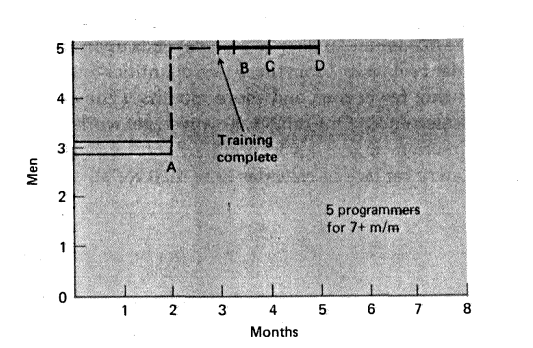
\includegraphics[scale=0.6]{MYTHICAL_MAN_MONTH_FIG_1.png}

Since the B milestone hasn’t been reached, there is temptation to repeat the cycle and add more manpower. Therein lies madness.

This assumes that only A  was misestimated. The less optimistic we are about the schedule, the more men we will want to add just to the original task. Without a doubt, the regenerative disaster will yield a poorer product, later, than would rescheduling with the original three men, unaugmented.

\newpage
\section{No Silver Bullet}

\subsection{Does It Have To Be Hard? Essential Difficulties}

The essence of a software entiy is a construct of interlocking concepts: data sets, relationship between data items, etc. This essence is abstract, in that the conceptual construct is the same under many representations. The hard part of building software is specification, design and testing of this conceptual construct, not the labor of representing it and testing it. If this is true, building software will always be hard. There is inherently no silver bullet. Let us consider the inherent properties of this essence of modern software system:

\begin{itemize}
    \item \textbf{Complexity} Software entities are more complex than any other human construct, because no two parts are alike. They also tend to have a very high number of states.This makes describing and testing them difficult. Because of these unique characteristics, when a system scales up it does it on a non linear complexity scale. This complexity is essential, you cannot abstract it without abstracting the essence of the system. Complexity problems lead to technical issues - harder team communication, schedule delays, product flaws, cost overrun- and management -controlling all the loose ends of the system- ones.
    \item \textbf{Conformity} Much of the previously mentioned complexity comes from previous instances of conformity from the software engineers themselves. Either conformation because they are new, or by conformation to previous terrible software interfaces.
    \item \textbf{Changeability} Sofware entities are subject to a lot of pressure to change. This is partly because the software embodies its function, and that is the part that is usually more pressured to change. Partly because it is much more mallable cost-wise (e.g. than a bulding). Software gets frequently changed because its function gets extended beyond the original domain. It can also change to adapt to new vehicles of opportunity (new technologies, infrastructure, etc.).
    \item \textbf{Invisibility} You cannot see software. Software structure diagrams ofter end up being several directed graphs, superimposed upon one another. As such, you cannot use powerful tools such as geometric abstractions. Imagine the plans for a building floor, you can see errors and omissions made just by seeing the plans. 
\end{itemize}

\subsection{Past Breakthroughs And How They Solved Accidental Difficulties}

\begin{itemize}
    \item \textbf{High-Level Languages}: A high-level language frees a program from much of its accidental complexity. The most a high-level language can do is to furnish all the constructs the programmer imagines in an abstract program. Then, the accidental complexity is eliminated because the language embodies the abstract construct -operations, data types, sequences- and not the lower concrete machine ones -registers, bits, disks-.
    \item \textbf{Time-Sharing}: Time sharing attacks a distinctly different difficulty: to shorten response times. It preserves inmediacy, allowing us to maintain an overview of complexity. The interruption of the minutae or thrust of the program idea caused by batch programming has a high cost associated to it, because we have to refresh later. This slow machine turnaround is an accidental difficulty.
    \item \textbf{Unified Programming Environments}: They attack the accidental difficulties of using programs together by providing integrated libraries, unfied file formats, filters.
\end{itemize}

\subsection{Hopes for the Silver}

\begin{itemize}
    \item \textbf{Ada and other high-level language advances}: Ada is a general purpose, high level languge that embodies the philosophy of modernization, abstract data types and hierarchical structuring. It won't be the silver bullet, since once the accidental complexities of the machine have been removed, the remaining ones are smaller (and their payoff less relevant).
    \item \textbf{Object-oriented programming}: We must distinguish to ideas here: abstract data types and hierarchical types (classes). The concept of the abstract data type is that an object's type should be defined by a name, a set of proper values and operations, rather than its storage structure (which should be hidden). Hierarchical types allow the definition of general interfaces that can be further refined by providing subordinate types. Each concept removes accidental difficulty from the process, allowing us to express the essence of the design without having to express massive amounts of syntactic material that adds no new information.
    \item \textbf{Artificial Intelligence}: Definition of AI-1: The use of computers to solve problems that could previously be solved only by human intelligence. Something can fit the definition of AI-1 today, but once we understand the problem and how it works, it won't fit anymore. Most of this work is problem specific and seems non transferrable to other fields without a lot of abstraction and creativity.
    \item \textbf{Expert Systems} (ES): An ES is a program containing a generalized inference engine and a rule base, designed to take input data and assumptions and explore the logical consequences through the inferences derivable from the rule base, yielding conclusions and advice, and being able to retrace its steps. Advantages over algorithms:
    \begin{enumerate}
        \item Inference engines are developed abstracted from the application, and can be reused easily.
        \item The changeable parts of the application are encoded in a uniform fashion, with tools for developing/testing the rule base. This regularizes much of the complexity of the application.
    \end{enumerate}
    The power of these programs comes from the separation between the engine and the application, and the ever growing and refined knowledge bases.
    Example: an imaginary testing advisor. As the knowledge base and inference engine being small and underdeveloped, it can only give rudimentary suggestions. As it is further expanded, it starts being more accurate and giving more precise and complex diagnostics. It can also be a tool that enforces good programming practices, generating a knowledge base as engineers create test cases. It is essential to, of course, have an expert first that guides the essence of the ES.
    \item \textbf{"Automatic" Programming}: The generation of a program for solving a problem from a statement of the problem specifications. Parnas argues that, in essence the solution method specification has to be given, not the problem-related one. Exceptions can be found, for example building generators to great advantage in sorting and differential equations. However, these applications need very favorable properties, and they also need problems readily characterized by few parameters, with many known methods of solution.
    \item \textbf{Graphical Programming}: Unfortunately, the flow chart is a \textbf{very} poor representation of software structure. Programmers tend to write them after writing the programs, rendering them useless as a high level abstraction. Software is also very difficult to visualize, as it's usually comprised of many, multi leveled, layered, directed graphs. Superimposed all these diagrams makes it hard to get a general-level view.
    \item \textbf{Program Verification}: Useful for, for example, secure operating system kernels. This verifcation does not mean error-proof systems, it only means that the system meets its own specifications. The hardest part of the software task is arriving at a complete and consistent specification, and much of the essence of building a program is the debugging of this specification.
    \item \textbf{Environments and Tools}: Benefits to gain: freedom from simple semantic and syntactic errors. The biggest gain will be the use of integrated database systems instead of having to keep everything on a single system. But by it's nature, the return from here will be marginal.
\end{itemize}

\subsection{Promising Attacks on the Conceptual Essence}

\begin{itemize}
    \item \textbf{Buy Versus Build}: The idea is to buy specific pieces of software for specific domain-based purposes instead of building your own . This products tend to be better documented and maintained, and delivery is usually immediate for as low a cost as a programmer year. The cost of software has always been development, not replication. The use of \textbf{N} copies of a software effectively multiplies the productivity of those developers by \textbf{N}. 
    
    Market-wise, there has been a huge change in the hardware/software ratio. Machines are much cheaper nowadays. As such, they are available to a massive audience that cannot afford custom payroll programs that slip easily into the computer hostile environment. In turn, they adapt their payroll procedures to the packages available in the market.
    
    Many users use computers to solve problems with electronic spreadsheets and simple DB systems, and yet many of them cannot write a single program. As such, \textbf{the single most software productivity strategy for man organizations today is to equip the computer- naive intellectual workers with personal computers and good generalized writing, drawing, file and spreadsheet programs, and turn them loose}.
    \item \textbf{Requirements Refinement and Rapid Prototyping}: The hardest part of building software is deciding what to build, since it is very hard to rectify later and cripples the system if done wrong. Clients do not know what they want, so iterative extraction and refinement of product requirements is essential.
    
    Therefore, one of the most promising efforts that attacks the essence of the software question is the development of approaches and tools for rapid prototyping of systems -simulating the interfaces and doing the main functions of the intended software- as part of the iterative specification of requirements. The assumption that one can specifcy a satisfactory system completely in advance, and later have it built and installed in one phase is fundamentally wrong.
    \item \textbf{Incremental Development-Grow, not Build, Software}: Instead of building software, we should use a "growing software" metaphor. Software should be "grown" with incremental development. First make it run, even if it does nothing. Then, you flesh it out bit by bit with rapid prototyping. This quick growth and iteration process skyrockets productivity and morale to unprecedented levels, since you have, at every stage, a working sytem. You can grow much more complex entities in four months than the ones you can build.
    \item \textbf{Great Designers}: Promoting good design practices is essential. This grows poor designs into good ones. However, \textbf{great} design comes from great people, since software construction is in itself a very creative process. Products built by great designers are faster, smaller, simpler, cleaner, and produced with less effort. The best effort we can mount is to grow great designers.
    
    To do this, one must identify top designers as early as possible. The best are often not the most experienced. Assign a career mentor to the designer and keep a solid career file. Devise and mantain a career development path for each prospect, including selected apprenticeships with top designers, courses, and advanced formal education, interprised with solo design and leadership challenges. Lastly, it is very important that you provide opportunities for these designers to interact with each other.
\end{itemize}

\newpage

\section{The Early History of Smalltalk}

\subsection{1960-66: Early OOP and Other Formative Ideas of the Sixties}

OOP came from two motivations: wanting to eliminate assignement and finding a better module scheme for complex systems involving hiding of details.

\subsubsection{Sketchpad and Simula}

Sketchpad was the invention of modern interactive computer graphics; things were described by making a "master drawing" that could produce "instance drawings"; control and dynamics were supplied by "constraints," also in graphical form, that could be applied to the masters to shape an inter-related parts. It also had pointers to procedures and using a process called reverse indexing to jump through them to routines. For a graphical reference, please see \textbf{figure \ref{fig:sketchpad}} at the end of the doc.

\begin{figure}[ht]
        % read manual to see what [ht] means and for other possible options
        \centering 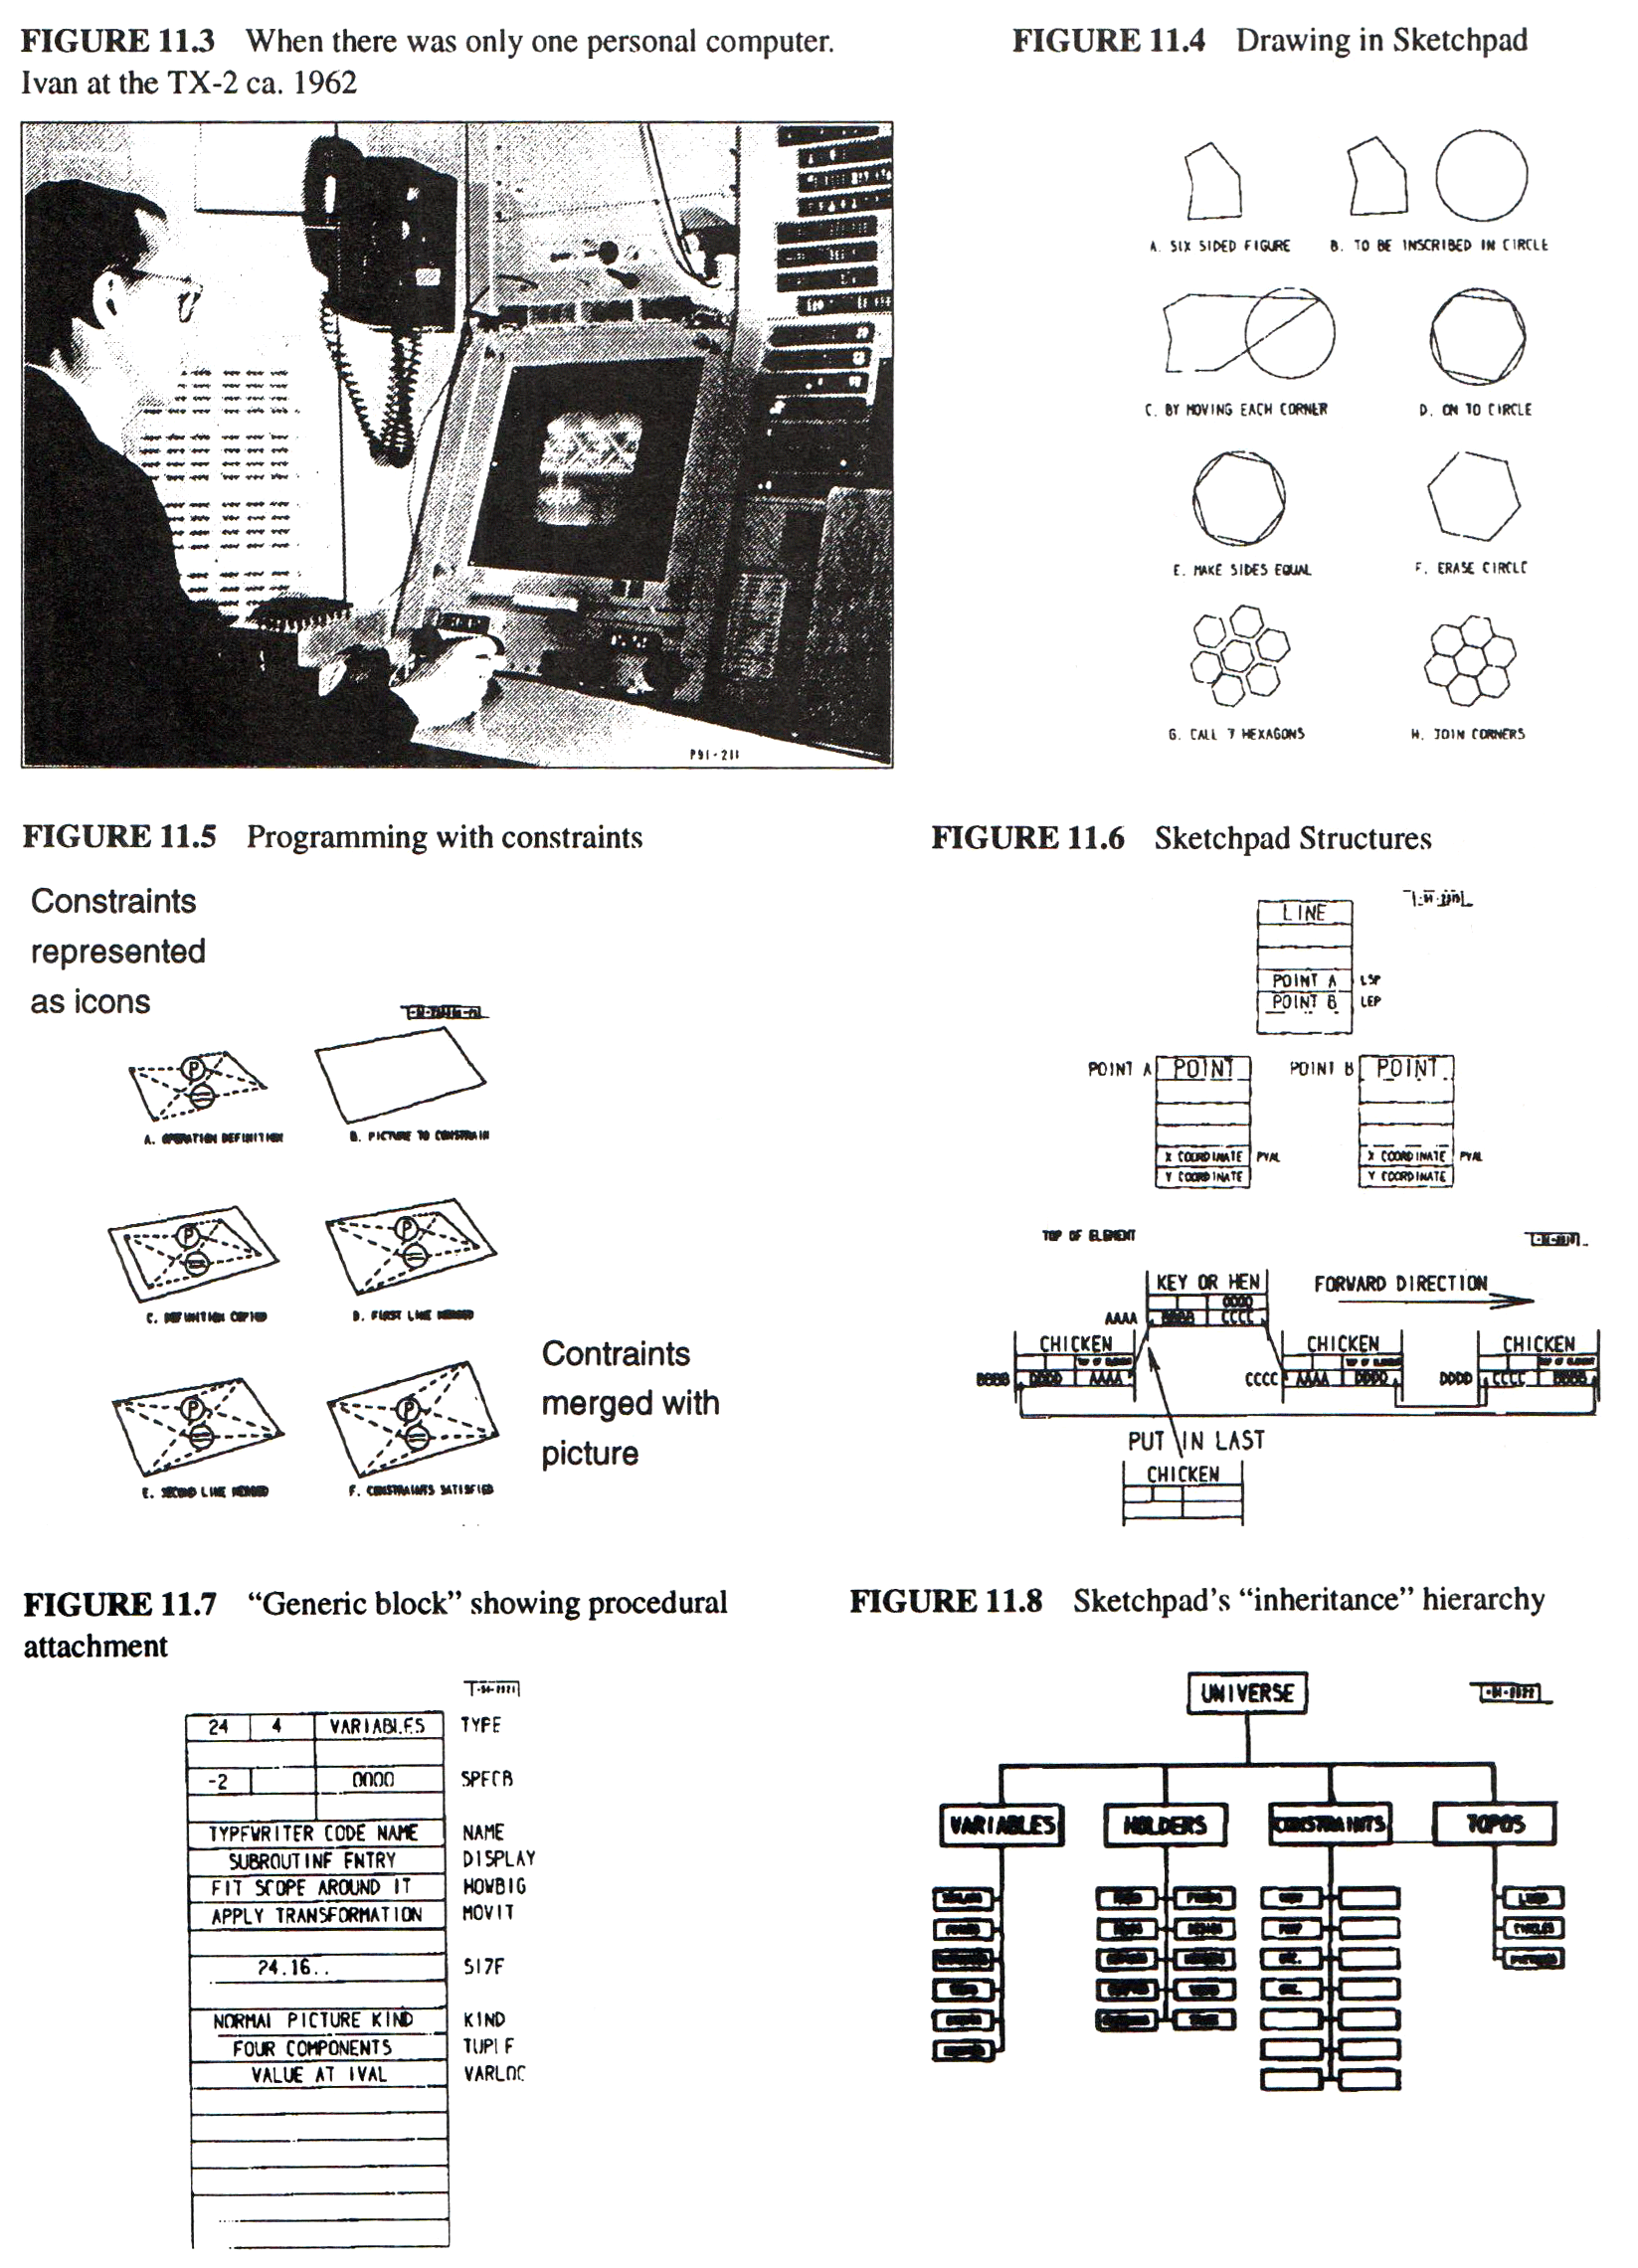
\includegraphics[scale=0.30]{SKETCHPAD.png}
        % note that in above figure file name, "sr_setup",
        % the file extension is missing. LaTeX is smart enough to find
        % apropriate one (i.e. pdf, png, etc.)
        % You can add this extention yourself as it seen below
        % both notations are correct but above has more flexibility
        %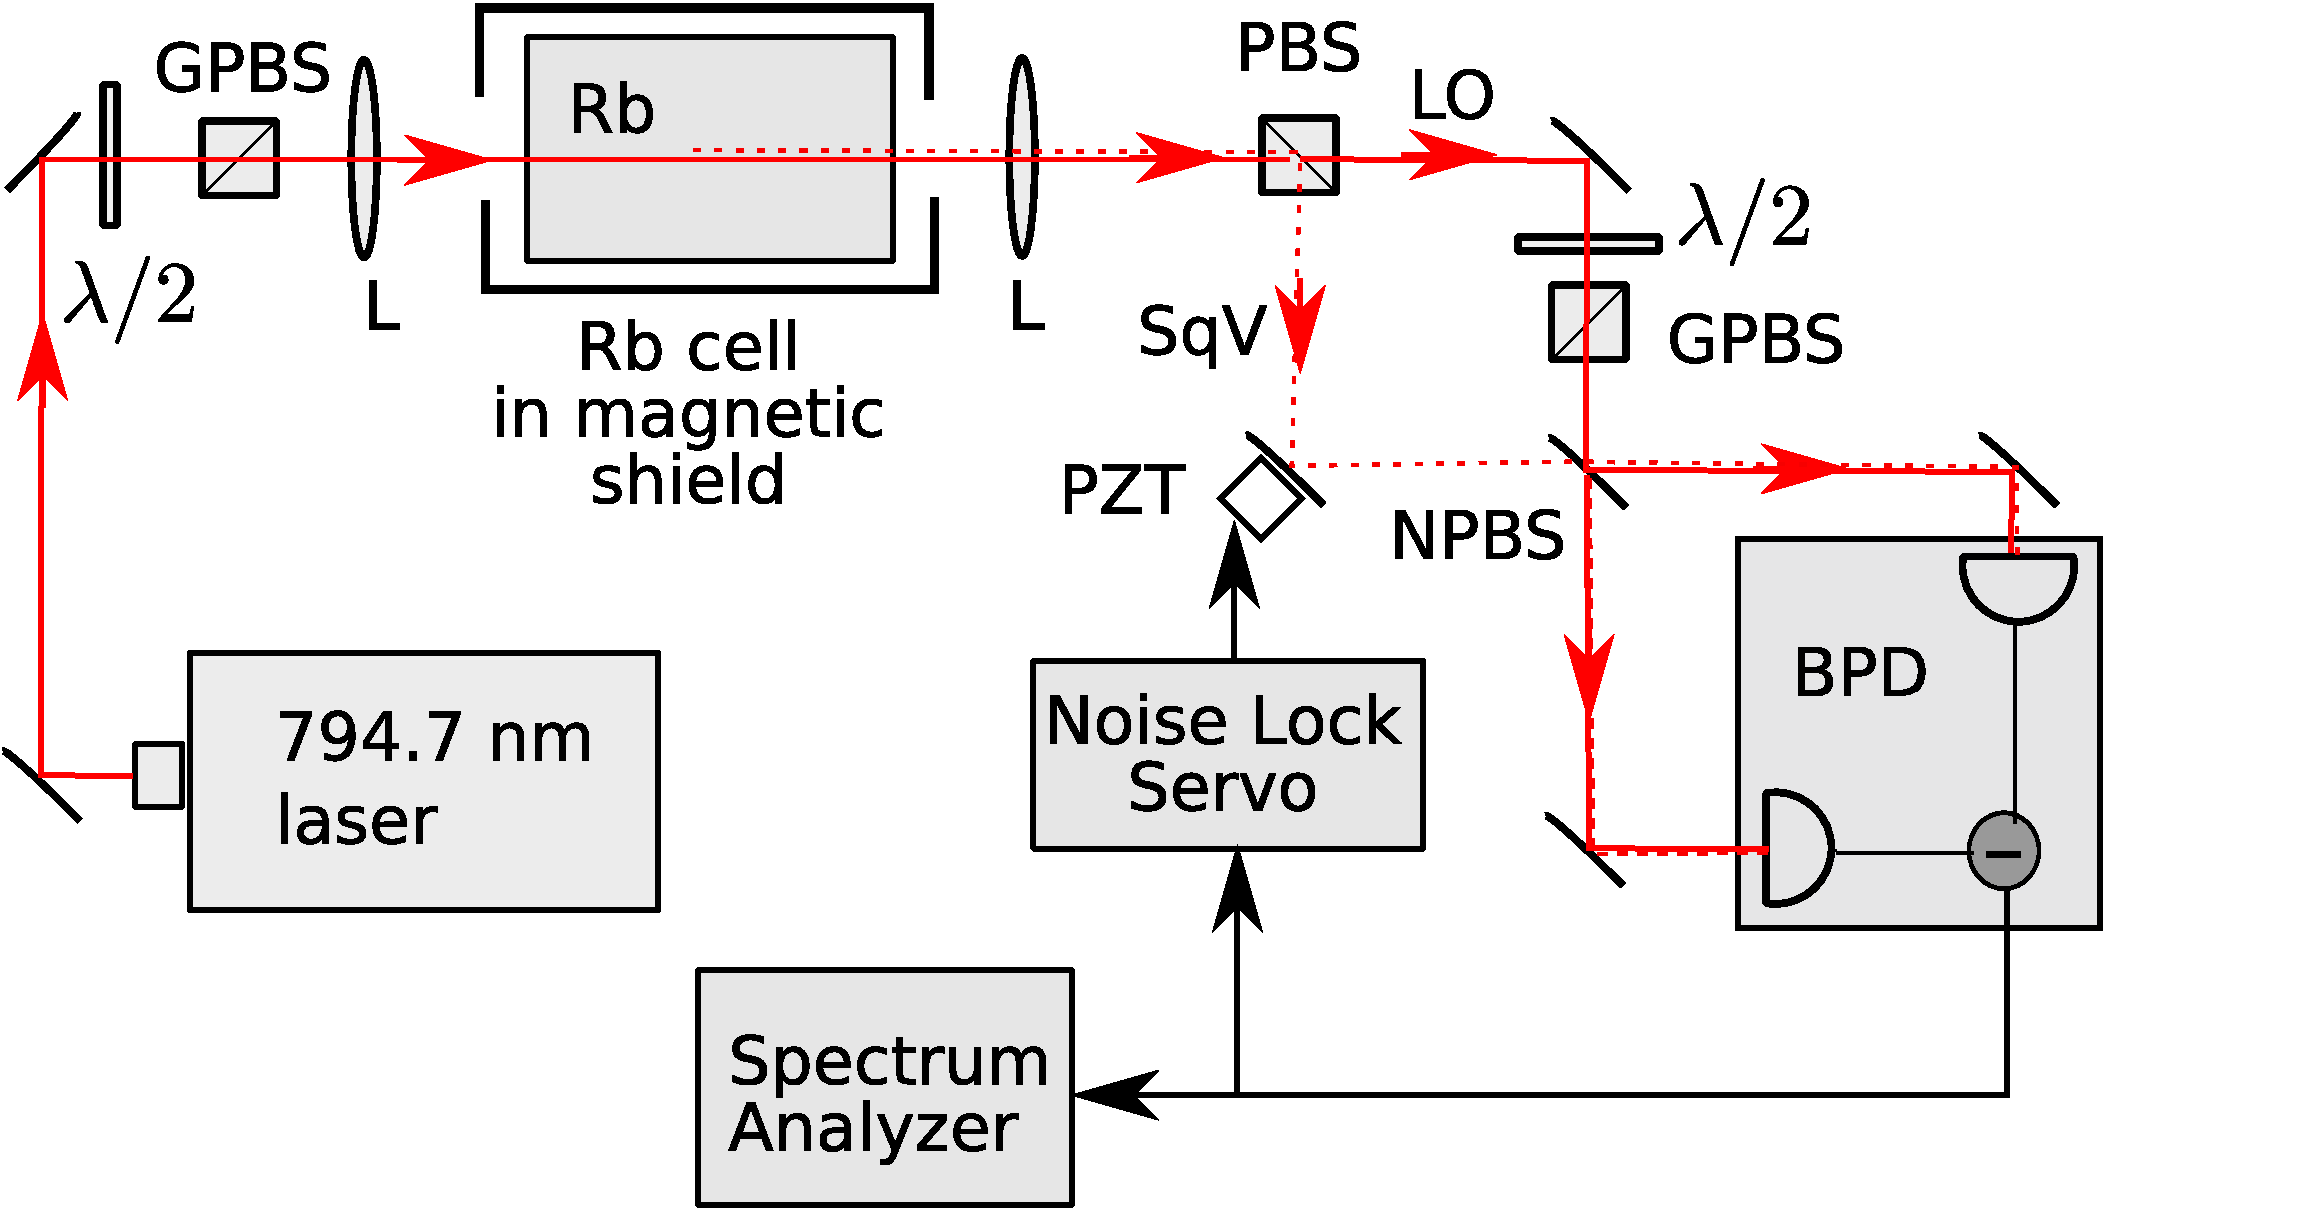
\includegraphics[width=1.0\columnwidth]{sr_setup.pdf}
        \caption{
                \label{fig:sketchpad} % spaces are big no-no withing labels
                % things like fig: are optional in the label but it helps
                % to orient yourself when you have multiple figures,
                % equations and tables
                Early History of Smalltalk: Sketchpad.
        }
\end{figure}

For Simula, the storage allocator part of the program was allocating structures very much like the instances of Sketchpad. There were descriptions that acted like masters and they could create instances, each of which was an independent entity. Simula was a procedural language for controlling Sketchpad-like objects, thus having considerably more flexibility than constraints.

\subsection{1967-69: The FLEX Machine, a First Attempt at an OOP-Based Personal Computer}

The FLEX Machine was a collaboration between Ed Cheadle and myself. We chose EULER as its language, since JOSS did not have enough computing power and aptitudes for simulating and extending -the main purpose of the FLEX Machine-. Because of the nature of the EULER compiler, the FLEX Machine could run byte-codes emulated in the longish slow microcode that was then possible. However, it required syntax concessions (e.g. "," could only be used in one role because the precedence scheme had no state space). We knew that the semantics of what was now called the FLEX language needed to be influenced more by Simula than by EULER.

\subsubsection{Doug Engelbart and NLS}

Doug's notion was that the destiny of oNLine Systems (NLS) was the "augmentation of human intellect" via an interactive vehicle navigating through concept space . What his system could do was incredible. Not just hypertext, but graphics, multiple panes, command input, interactive collaborative work, etc. One of the interesting features of NLS was that its user interface was parametric and could be supplied by the end user in the form of a "grammar of interaction" given in their compiler-compiler TreeMeta. Unfortunately, these grammars forced the user to be in a system state which required getting out of before any new kind of interaction could be done. A much "flatter" interface was needed.

\subsubsection{FLEX Machine Concepts}

Object references were handled on the FLEX Machine as a generalization of B5000 descriptors. A FLEX descriptor contained two pointers: the first to the "master" of the object, and the second to the object instances. A different method was taken for handling generalized assignment. For example: a[55] := 0 needed to be something like: a(55, ':=', 0), so it would look at all the relevant operands first. From this we can conclude that := is not an operator, but a kind of index that can select a behavior from a complex object. \textbf{It is here that we can see that objects need to privately own all of their behaviors: that objects are a kind of mapping whose values are its behaviors}. For a graphical reference, please see \textbf{figure \ref{fig:flex_1}} at the end of the doc.

\begin{figure}[ht]
        % read manual to see what [ht] means and for other possible options
        \centering 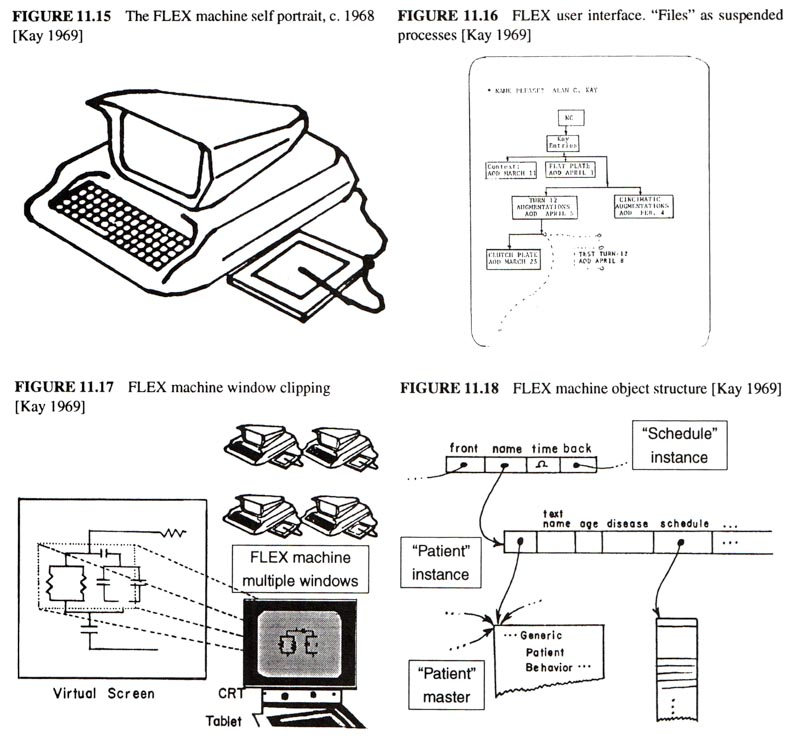
\includegraphics[scale=0.65]{FLEX_MACHINE_1.jpg}
        % note that in above figure file name, "sr_setup",
        % the file extension is missing. LaTeX is smart enough to find
        % apropriate one (i.e. pdf, png, etc.)
        % You can add this extention yourself as it seen below
        % both notations are correct but above has more flexibility
        %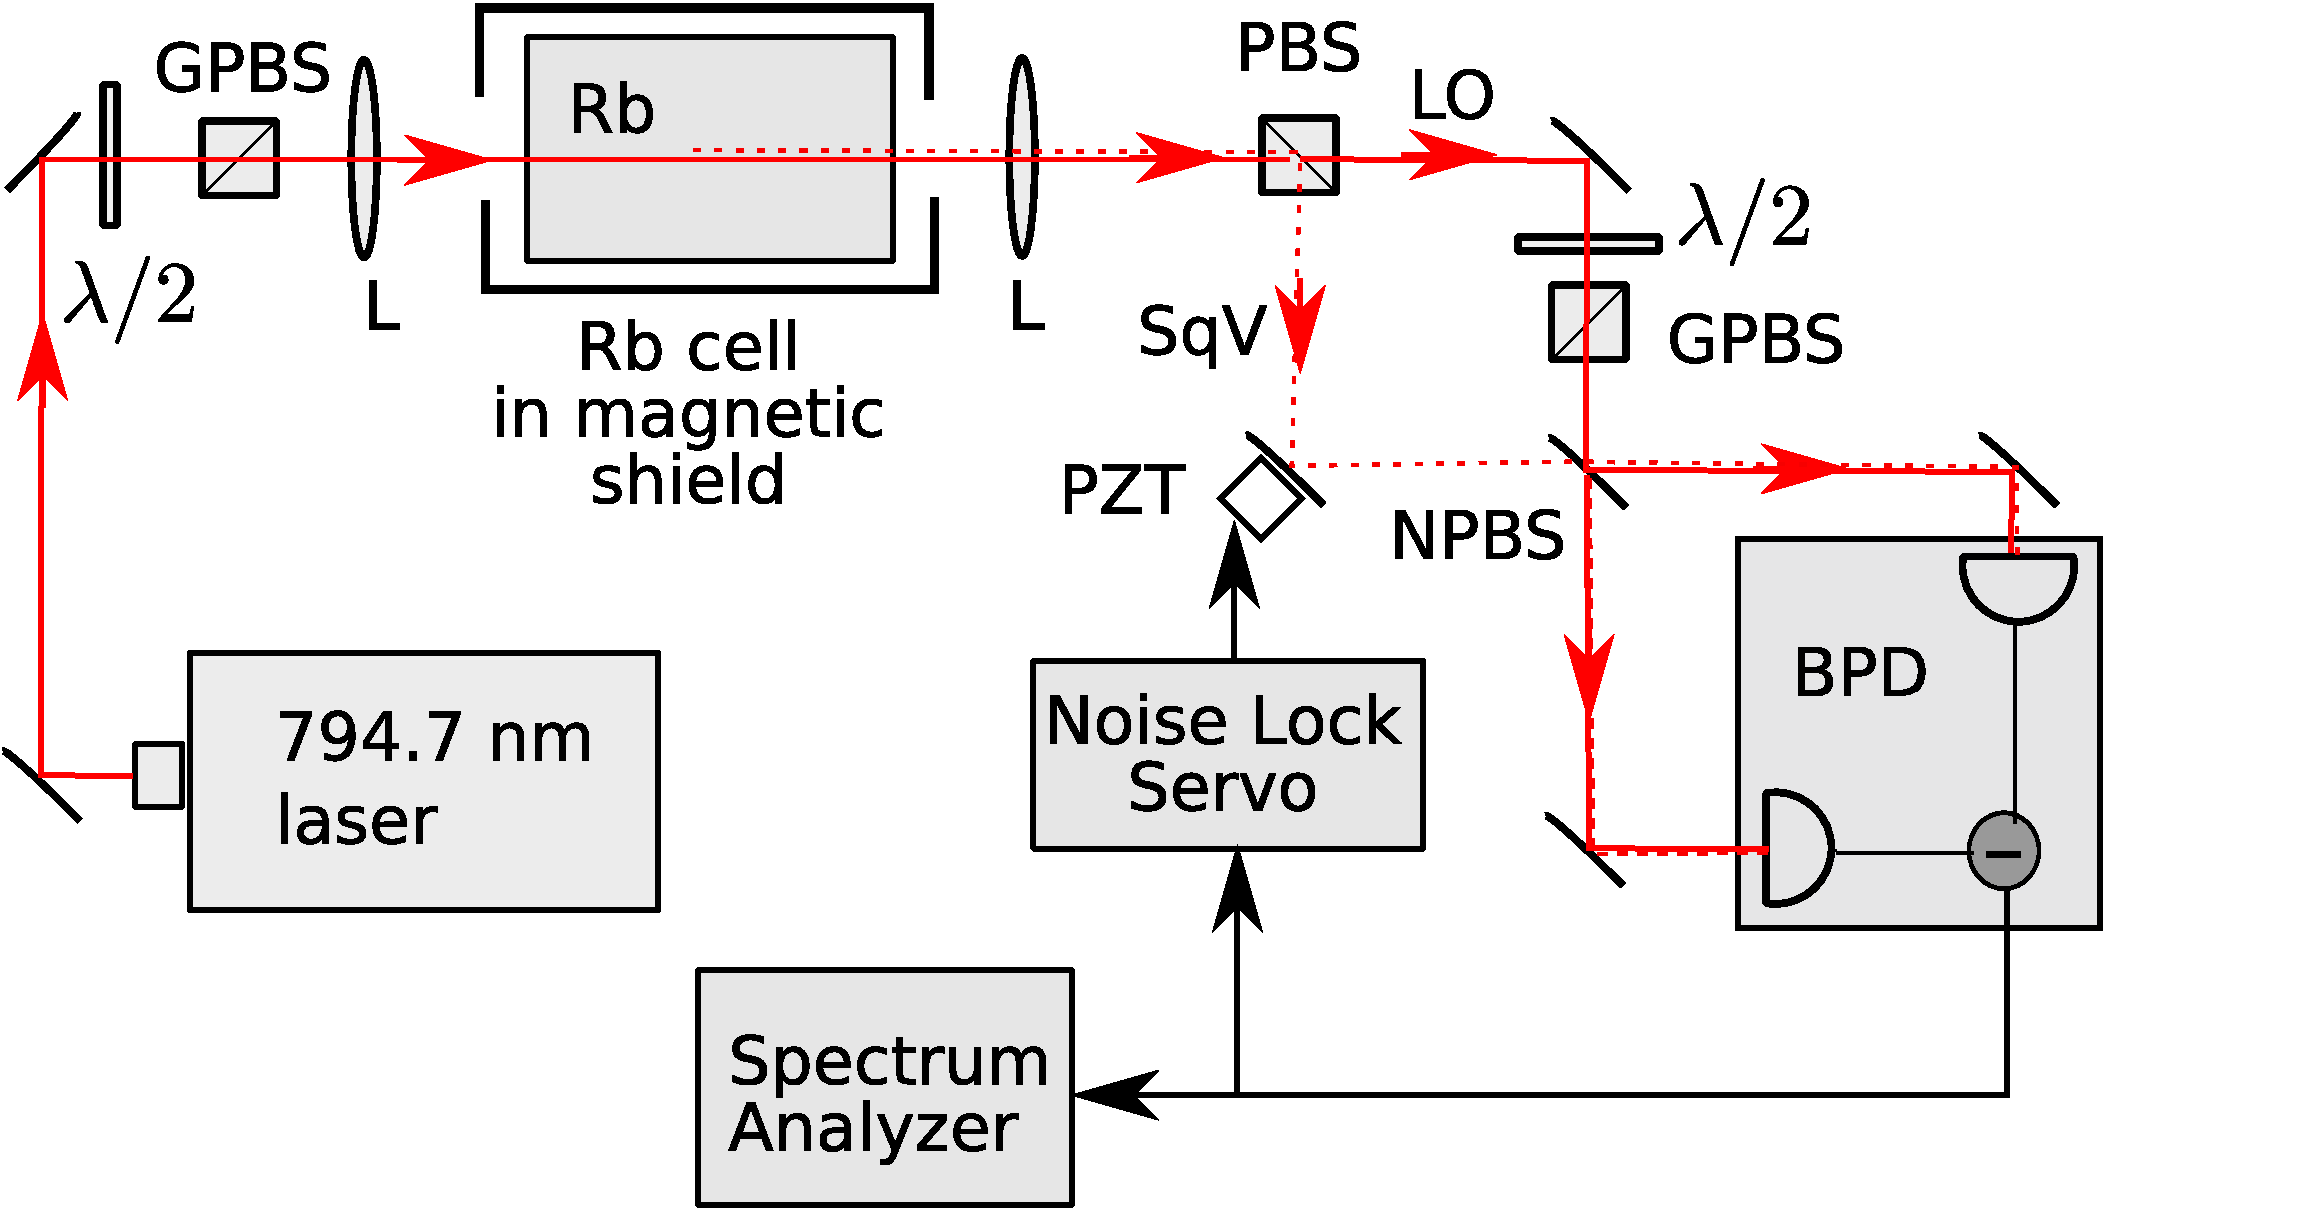
\includegraphics[width=1.0\columnwidth]{sr_setup.pdf}
        \caption{
                \label{fig:flex_1} % spaces are big no-no withing labels
                % things like fig: are optional in the label but it helps
                % to orient yourself when you have multiple figures,
                % equations and tables
                Flex Machine 1.
        }
\end{figure}

Another control structure in FLEX is called \textbf{when}.  Its boolean expression was compiled into a "tournament sort" tree that cached all possible intermediate results. The relevant variables were threaded through all of the sorting trees in all of the whens so that any change only had to compute through the necessary parts of the booleans. However, this was beyond the scope of FLEX and needed to wait for a better architecture, since, for example, part of the boolean had to be used just to check the contexts.

\subsubsection{Dynabook}

GRAIL was the graphical follow up to JOSS, following the same principles. Now the collision of the FLEX machine, the flat-screen display, GRAIL, Barton's "communications" talk, McLuhan, and Papert's work with children all came together to form an image of what a personal computer really should be: the Dynabook.

 I wanted the Dynabook concept to embody the learning theories of Jerome Bruner and some of what Seymour Papert— who had studied with developmental psychologist Jean Piaget and who was one of the inventors of the Logo programming language — was proposing. Now, this concept was created two years before the founding of Xerox PARC. The ideas led to the development of the Xerox Alto prototype, which was originally called “the interim Dynabook”. It embodied all the elements of a graphical user interface, or GUI, as early as 1972. The software component of this research was Smalltalk, which went on to have a life of its own independent of the Dynabook concept. The hardware on which the programming environment ran was relatively irrelevant.

\subsubsection{LISP and it's Inspiration for Smalltalk}

The biggest hit for me while at SAIL in late '69 was to really understand LISP. The pure language was supposed to be based on functions, but its most important components—such as lambda expressions, quotes, and conds—were not functions at all, and instead were called special forms. Landin and others had been able to get quotes and conds in terms of lambda by tricks that were variously clever and useful, but the flaw remained in the jewel. In the practical language things were better. There were not just EXPRs (which evaluated their arguments), but FEXPRs (which did not). My next question was, why on earth call it a functional language? Why not just base everything on FEXPRs and force evaluation on the receiving side when needed? I could never get a good answer, but the question was very helpful when it came time to invent Smalltalk, because this started a line of thought that said "take the hardest and most profound thing you need to do, make it great, and then build every easier thing out of it". That was the promise of LISP and the lure of lambda—needed was a better "hardest and most profound" thing. Objects should be it.

\subsection{1970-72: Xerox PARC: KiddiKomp, miniCOM, and Smalltalk-71}

\subsubsection{Simulation LOGO}

In July 1970, Xerox, at the urging of its chief scientist Jack Goldman, decided to set up a long range research center in Palo Alto, California. There, I immediately started working up a new version of the KiddiKomp that could be made in enough quantity to do experiments leading to the user interface design for the eventual notebook. I still liked pattern-directed approaches and OOP so I came up with a language design called "Simulation LOGO" or SLOGO for short (I had a feeling the first versions might run nice and slow). This was to be built into a SONY "tummy trinitron" and would use a coarse bit-map display and the FLEX machine rubber tablet as a pointing device.

\subsubsection{LISP and It's Inspiration for the KiddiKomp}

 One little incident of LISP beauty happened when Allen Newell visited PARC with his theory of hierarchical thinking and was challenged to prove it. He was given a programming problem to solve. The problem was: given a list of items, produce a list consisting of all of the odd indexed items followed by all of the even indexed items. Because of Newell's internal programming language, he got into quite a struggle to do the program. In 2 seconds I wrote down:

\textit{oddsEvens(x) = append(odds(x), evens(x))}

\textit{where odds(x) = if null(x) ∨ null(tl(x)) then x else hd(x) \& odds(ttl(x))}
                  
\hspace{30 pt} \textit{evens(x) = if null(x) ∨ null(tl(x)) then nil else odds(tl(x))}

This characteristic of writing down many solutions in declarative form and have them also be the programs is part of the appeal and beauty of this kind of language. This incident and others like it made paramount that any tool for children should have great thinking patterns and deep beauty "built-in." 

\subsubsection{MiniCOM and the Birth of Smalltalk}

In the summer of '71 I refined the KiddiKomp idea into a tighter design called miniCOM. It used a bit-slice approach like the NOVA 1200, had a bit-map display, a pointing device, a choice of "secondary" (really tertiary) storages, and a language I now called "Smalltalk"—as in "programming should be a matter of ..." and "children should program in ...". For a graphical reference, please see \textbf{figure \ref{fig:minicom}} at the end of the doc.

\begin{figure}[ht]
        % read manual to see what [ht] means and for other possible options
        \centering 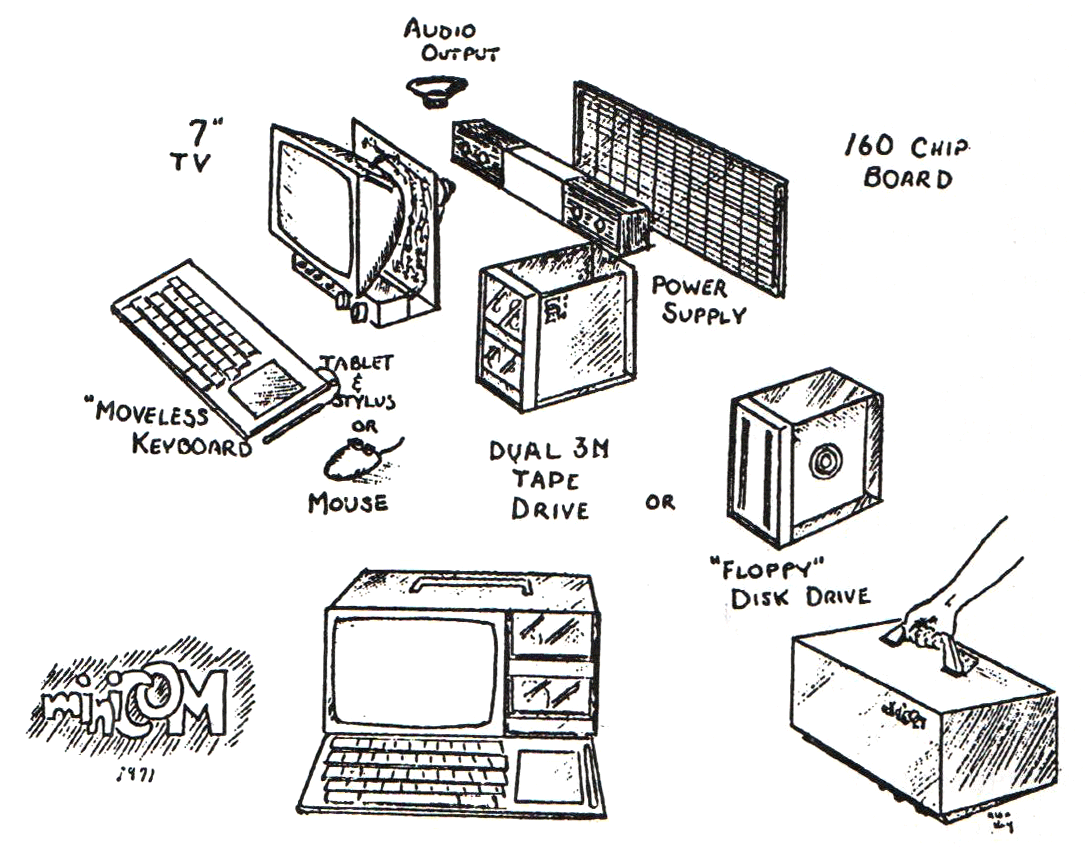
\includegraphics[scale=0.5]{MINICOM.png}
        % note that in above figure file name, "sr_setup",
        % the file extension is missing. LaTeX is smart enough to find
        % apropriate one (i.e. pdf, png, etc.)
        % You can add this extention yourself as it seen below
        % both notations are correct but above has more flexibility
        %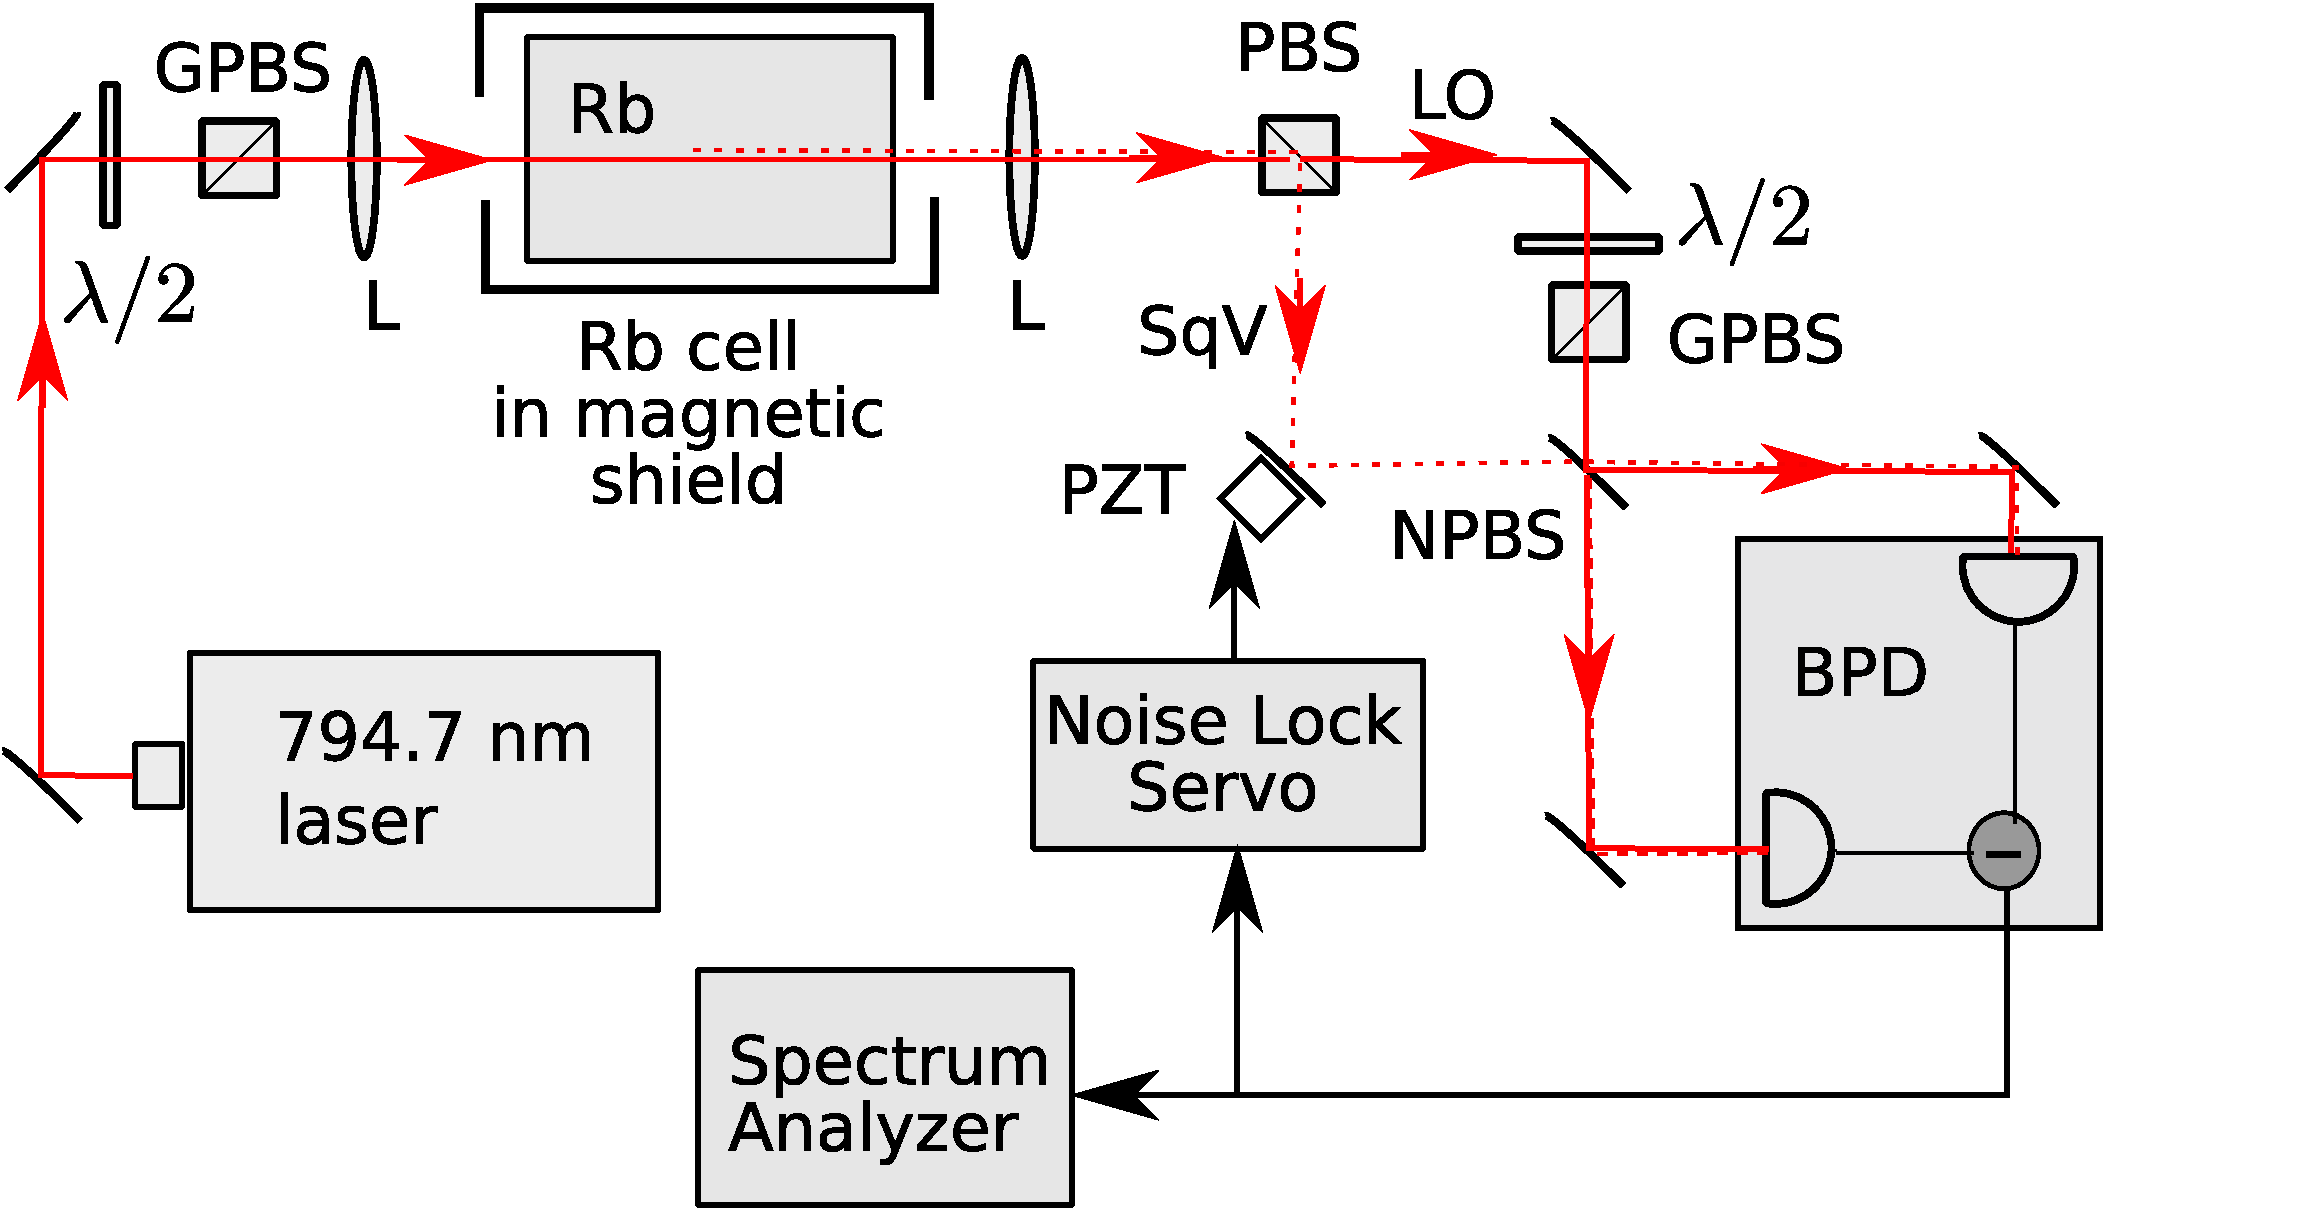
\includegraphics[width=1.0\columnwidth]{sr_setup.pdf}
        \caption{
                \label{fig:minicom} % spaces are big no-no withing labels
                % things like fig: are optional in the label but it helps
                % to orient yourself when you have multiple figures,
                % equations and tables
                MiniCOM.
        }
\end{figure}

\subsubsection{Smalltalk-71}

 It was a kind of parser with object-attachment that executed tokens directly. The patterned front-end allowed simple extension, patterns as "data" to be retrieved, a simple way to attach behaviors to objects, and a rudimentary but clear expression of its eval in terms that I thought children could understand after a few years experience with simpler programming. Program storage was sorted into a discrimination net and evaluation was straightforward pattern-matching. For various Smalltalk-71 example programs, please see \textbf{figure \ref{fig:smalltalk_71}} at the end of the doc.
 
 \begin{figure}[ht]
        % read manual to see what [ht] means and for other possible options
        \centering 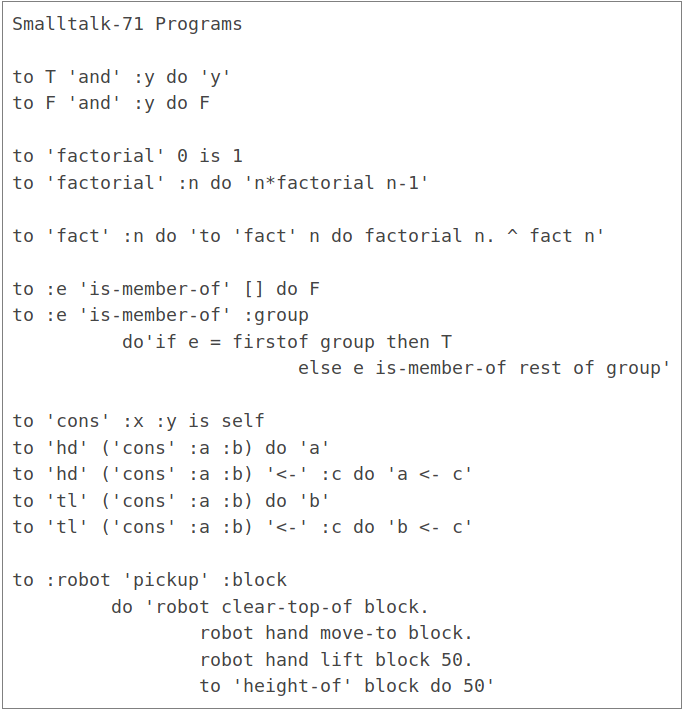
\includegraphics[scale=0.75]{SMALLTALK_71.png}
        % note that in above figure file name, "sr_setup",
        % the file extension is missing. LaTeX is smart enough to find
        % apropriate one (i.e. pdf, png, etc.)
        % You can add this extention yourself as it seen below
        % both notations are correct but above has more flexibility
        %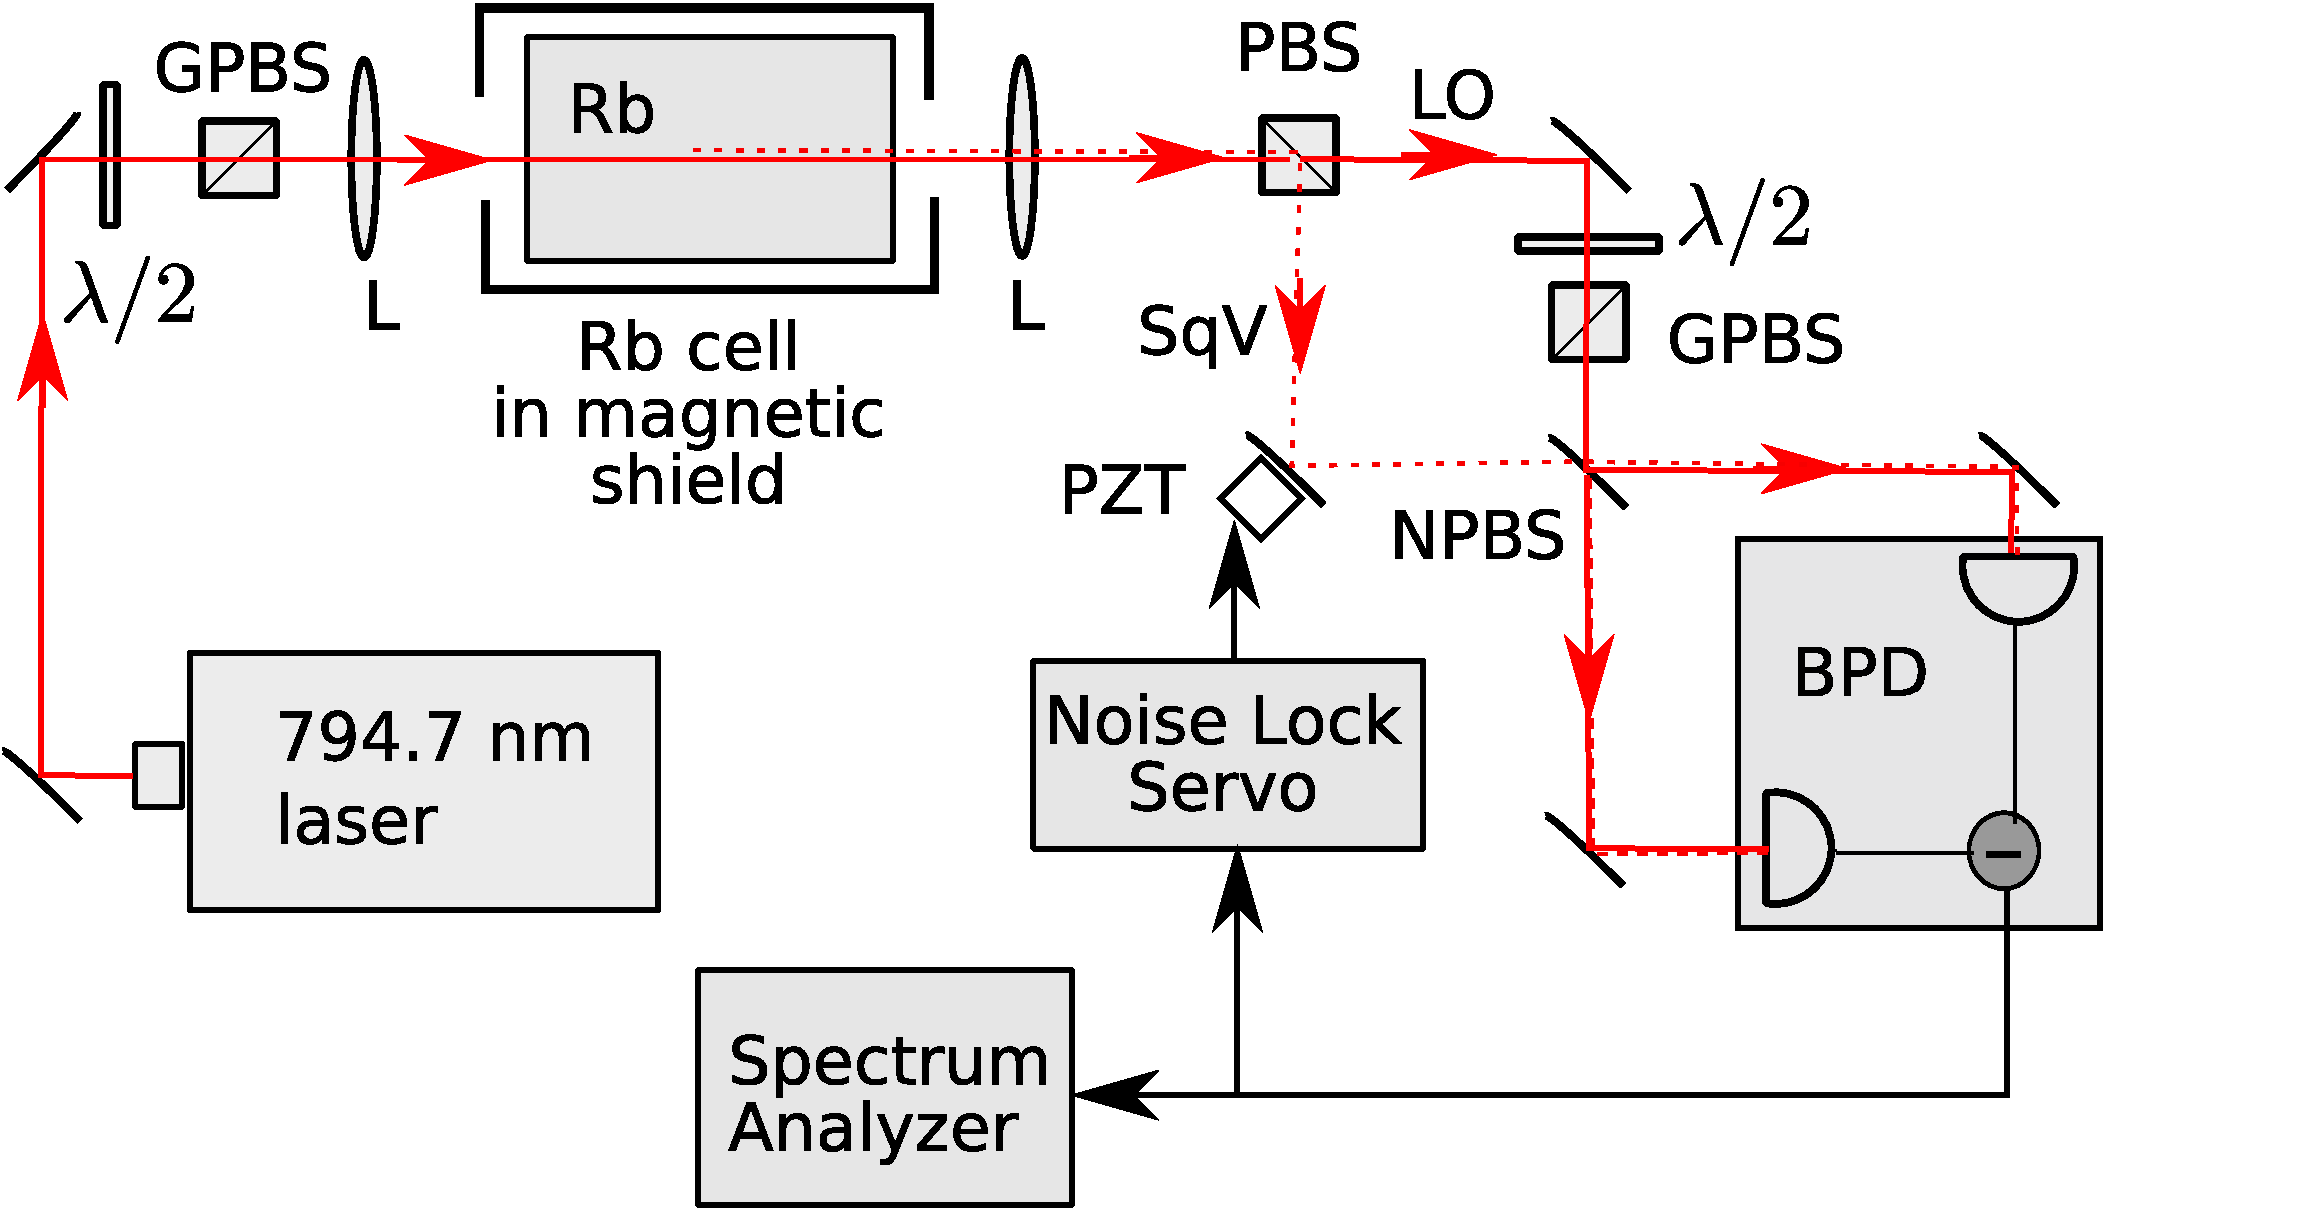
\includegraphics[width=1.0\columnwidth]{sr_setup.pdf}
        \caption{
                \label{fig:smalltalk_71} % spaces are big no-no withing labels
                % things like fig: are optional in the label but it helps
                % to orient yourself when you have multiple figures,
                % equations and tables
                Smalltalk-71 programs.
        }
\end{figure}

 A problem carried from LISP made me realize that we needed complete control over what was passed in a message send. In particular, \textit{when} and in \textit{what environment} did expressions get evaluated? Dave Fisher introduced the concept of \textbf{reflective design} to solve this: Associating the proper global state link with expressions and functions that are to be evaluated later so that the free variables referenced are the ones that were actually implied by the static language. 
 
 Putting this together with the FLEX models suggested that all that should be required for "doing OOP right" would be to handle the mechanics of invocations between modules without having to worry about the details of the modules themselves. The difference between LISP and OOP would then be what the modules could contain. A universal module (object) reference —ala B5000 and LISP—and a message holding structure that could be used by all would do the job. If all of the fields of a messenger structure were enumerated according to this view, we would have a stack similar to the one found in \textbf{figure \ref{fig:B5000_stack}}.

 \begin{figure}[ht]
        % read manual to see what [ht] means and for other possible options
        \centering 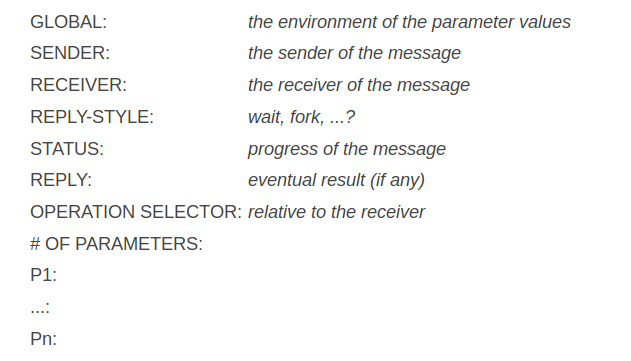
\includegraphics[scale=0.85]{B5000_STACK.png}
        % note that in above figure file name, "sr_setup",
        % the file extension is missing. LaTeX is smart enough to find
        % apropriate one (i.e. pdf, png, etc.)
        % You can add this extention yourself as it seen below
        % both notations are correct but above has more flexibility
        %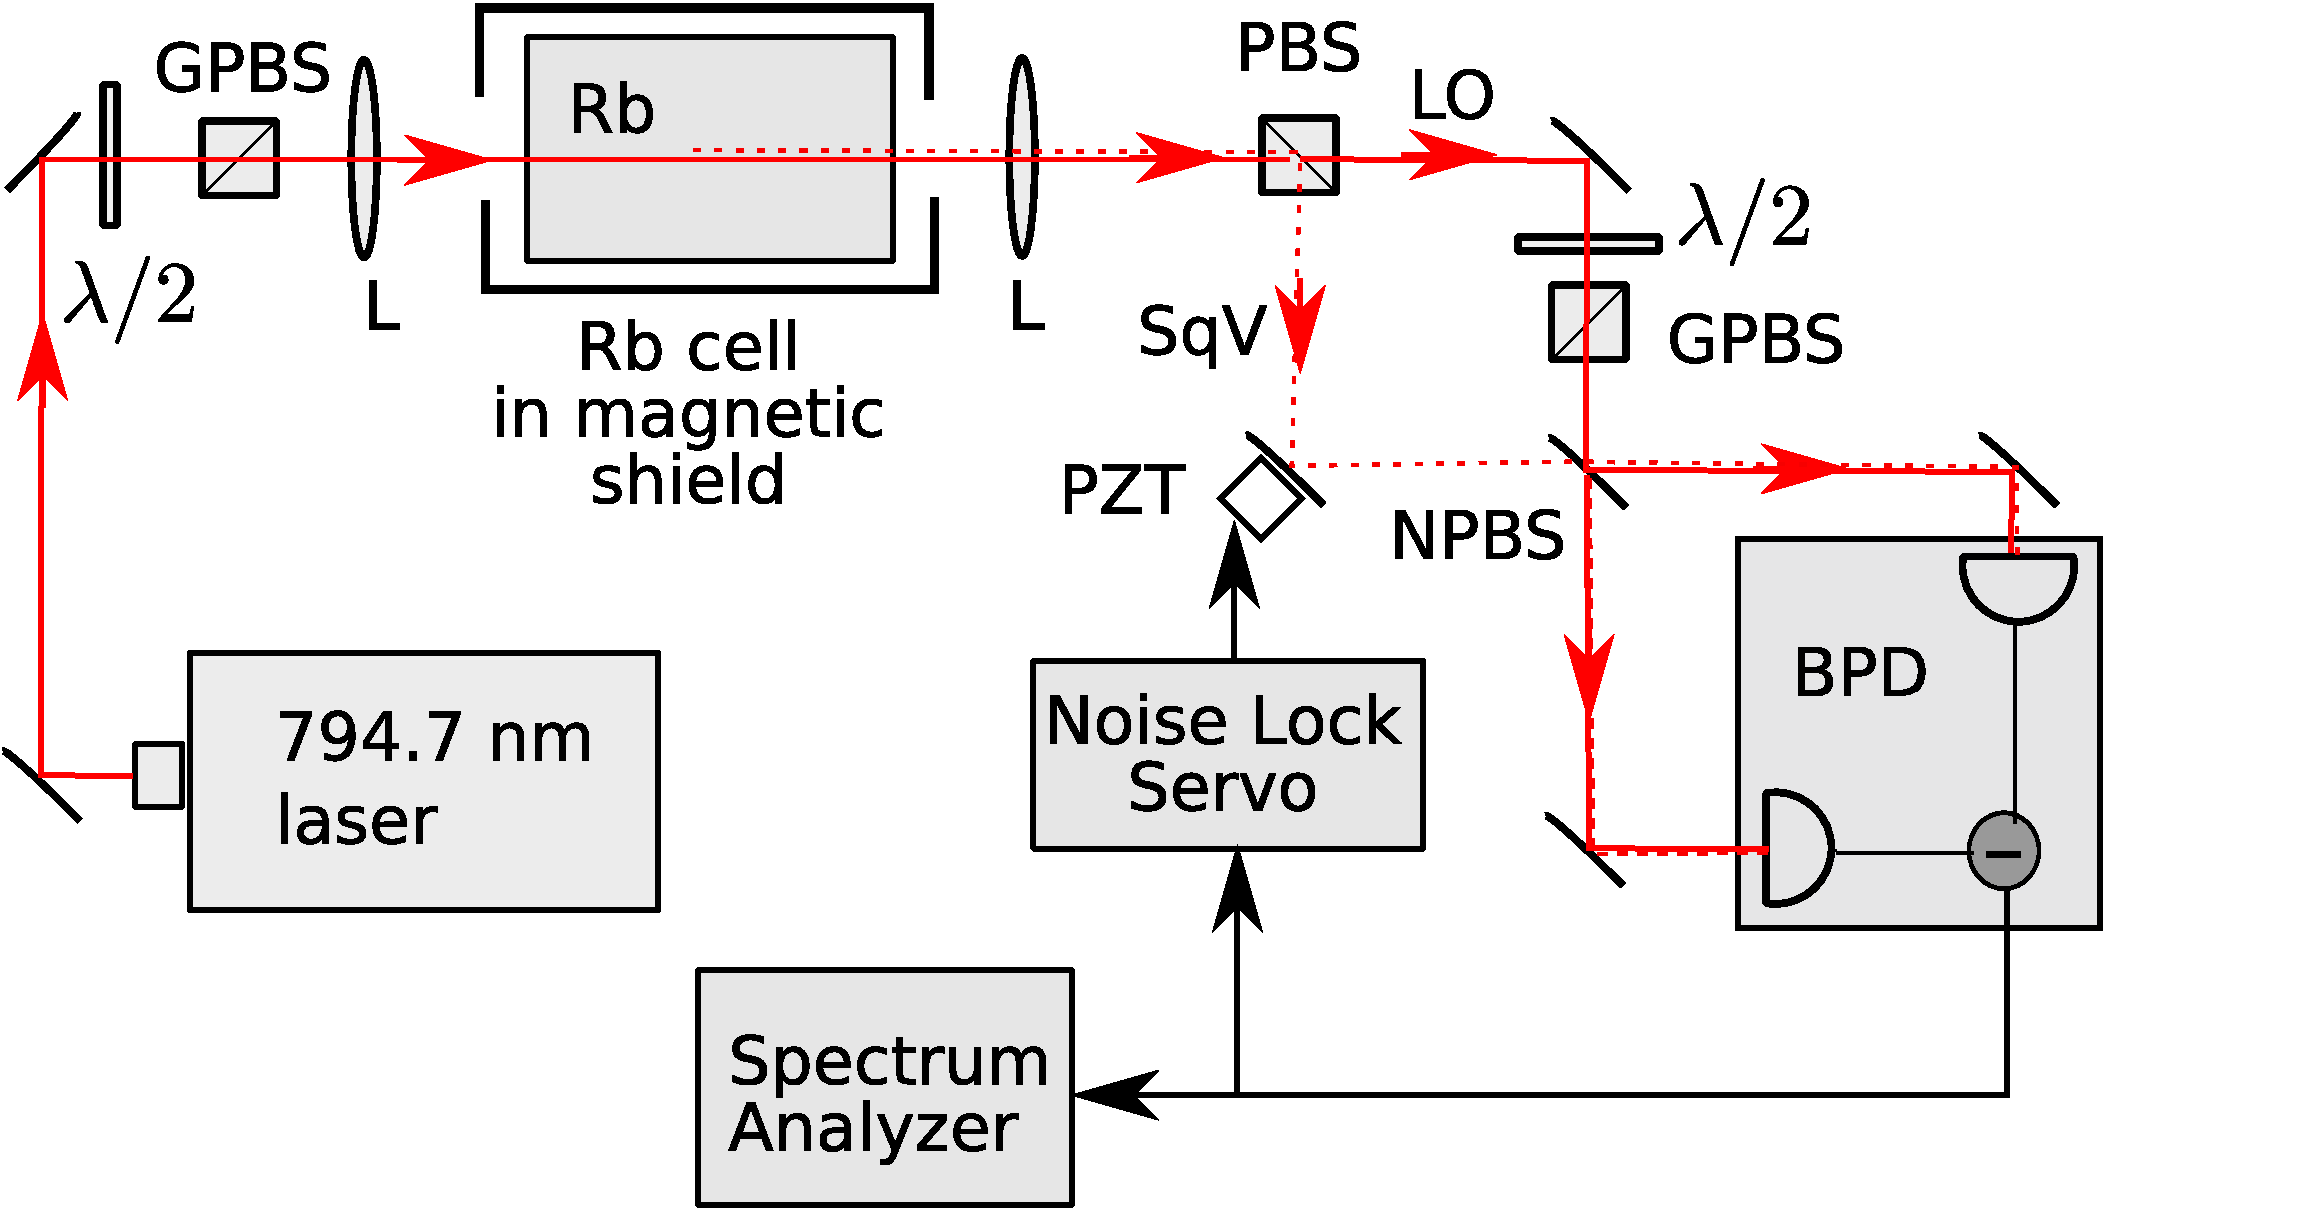
\includegraphics[width=1.0\columnwidth]{sr_setup.pdf}
        \caption{
                \label{fig:B5000_stack} % spaces are big no-no withing labels
                % things like fig: are optional in the label but it helps
                % to orient yourself when you have multiple figures,
                % equations and tables
                Example Stack.
        }
\end{figure}

\subsubsection{Improvements on the Display}

One of my continual worries at this time was about the size of the bit-map display. Even if a mixed mode was used (between fine-grained generated characters and coarse-grained general bit-map for graphics) it would be hard to get enough information on the screen. To investigate the use of video as a display medium, Bill English and Butler Lampson specified an experimental character generator for the POLOS (PARC OnLine Office System) terminals. The character generator's font memory turned out to be large enough to simulate a bit-map display if one displayed a fixed "strike" and wrote into the font memory

I got Steve Purcell, a summer student from Stanford, to build my design for bit-map painting so the kids could sketch as well as display computer graphics. John Shoch built a line drawing and gesture recognition system that was integrated with the painting. Bill Duvall of POLOS built a miniNLS that was quite remarkable in its speed and power. The first overlapping windows started to appear. Bob Shur built a 2½D animation system.

\subsubsection{Advancements on Education}

I also took another pass at the language for the kids. Jeff Rulifson was a big fan of Piaget (and semiotics) and we had many discussions about the "stages" and what iconic thinking might be about. After reading Piaget and especially Jerome Bruner, I was worried that the directly symbolic approach taken by FLEX, LOGO (and the current Smalltalk) would be difficult for the kids to process since evidence existed that the symbolic stage (or mentality) was just starting to switch on. In fact, all of the educators that I admired (including Montessori, Holt, and Suzuki) all seemed to call for a more figurative, more iconic approach. Rudolph Arnheim [Arnheim 69] had written a classic book about visual thinking, and so had the eminent art critic Gombrich [Gombrich **]. It really seemed that something better needed to be done here. GRAIL wasn't it, because its use of imagery was to portray and edit flowcharts, which seemed like a great step backwards. But Rovner's AMBIT-G held considerably more promise [Rovner 68]. It was kind of a visual SNOBOL [Farber 63] and the pattern matching ideas looked like they would work for the more PLANNERlike scheme I was using.


\subsection{1972-76: The first real Smalltalk (-72), its birth, applications, and improvements}

\subsubsection{Early Versions}

 The major differences from the official Smalltalk-72 of a little bit later were that in the first version symbols were byte-coded and the receiving of return-values from a send was symmetric (receipt could be like parameter binding). This was particularly useful for the return of multiple values. This was abandoned in favor of a more expression-oriented functional return style.

Only a few days later, Ingalls showed me the scheme working on the NOVA. He had coded it up (in BASIC!). It evaluated 3+4 very slowly but the answer always came out 7. Ingalls loved to bootstrap on a system that "always ran," and over the next ten years he made at least 80 major releases of various flavors of Smalltalk.

In November, I presented these ideas and a demonstration of the interpretation scheme to the MIT AI lab. This eventually led to Carl Hewitt's more formal "Actor" approach. In the first Actor paper the resemblance to Smalltalk is at its closest. The paths later diverged, partly because we were much more interested in making things than theorizing, and partly because we had something no one else had: Chuck Thacker's Interim Dynabook (the "ALTO").

\subsubsection{The Interim Dynabook}

Just before Chuck started work on the machine I gave a paper to the National Council of Teachers of English on the Dynabook and its potential as a learning and thinking amplifier—the paper was an extensive rotogravure of "20 things to do with a Dynabook". After a while, due to some bad press, executive "X" came back from his "task force" and tried to kill the project, fortunately failing to do so in the end.

In April 1973, the first Interim Dynabook -BILBO \ref{fig:bilbo}- was a reality. It featured a coroutine architecture (doing things asynchronously in a sequential manner). Lookaside logic scanned the flags while the current instruction was executing and picked the highest priority program counter to fetch from next. And so, the machine never had to wait.
 \begin{figure}[ht]
        \centering 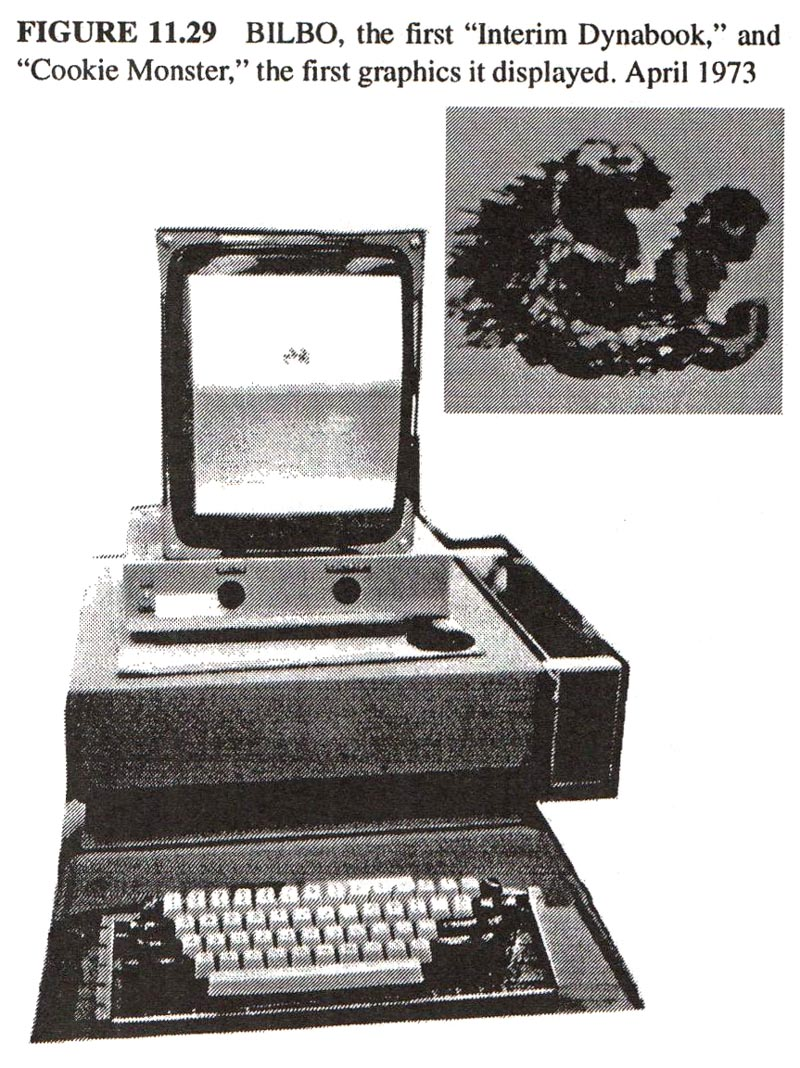
\includegraphics[scale=0.45]{BILBO.jpg}
        \caption{
                \label{fig:bilbo}
                The first Interim Dynabook.
        }
\end{figure}

\subsubsection{Smalltalk's Main Ideas}

\begin{enumerate}
    \item Everything is an object.
    \item Objects communicate by sending and receiving messages (in terms of objects).
    \item Objects have their own memory (in terms of objects).
    \item Every object is an instance of a class (which must be an object).
    \item The class holds the shared behavior for its instances (in the form of objects in a program list).
    \item To eval a program list, control is passed to the first object and the remainder is treated as its message.
\end{enumerate}

The \textbf{first three principles} are what objects "are about"—how they are seen and used from "the outside." These did not require any modification over the years. \textbf{The last three} —objects from the inside— were tinkered with in every version of Smalltalk.

 Point number 6 implies a LISPlike universal syntax, but with the receiving object as the first item followed by the message. An example operation of (ci <- de) with integers could be 3+4. This would translate to 3 being the reciever and  "+4" being the message. Other examples  with strings and matrixes would be:
 
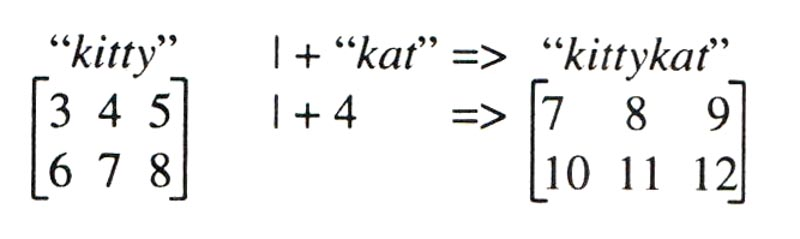
\includegraphics[scale=0.3]{KITTYKAT.jpg}

\subsubsection{Development of the Smalltalk-72 System and Applications}

\textbf{Overlapping windows} were the first project tackled.	In the end, we opted for the style that is still in use today, which is more like "$2^{1/4}$ D" . Windows were perhaps the most redesigned and reimplemented class in Smalltalk because we didn't quite have enough compute power to just do the continual viewing to "world coordinates" and refreshing we wanted.

One of the next classes to be implemented on the Interim Dynabook (after the basics of numbers, strings, etc.) was an object-oriented version of the \textbf{LOGO turtle}. This could make many turtle instances that were used both for drawing and as a kind of value for graphics transformations \ref{fig:windows_and_turles}.

Larry Tesler did not like the modiness and general approach of NLS, and he wanted both to show the former NLSers an alternative and to conduct some user studies about editing. This led to his programming \textbf{miniMOUSE} in Smalltalk, the first real WYSIWYG galley editor.

There were several other inventions along the way. \textbf{Findit}, a "retrieval by example" interface that used the analogy of classes to their instances to form retrieval requests. There was also \textbf{OPUS}, the first real-time score capturing system (like a metronome but with very different logic). Finally, there was \textbf{SHAZAM}, a marvelously capable and simple animation system.

The main thesis project during this time was Dave Smith's \textbf{PYGMALION}, an essay into iconic programming. One programmed by showing the system how changes should be made, much as one would illustrate on a blackboard with another programmer. 

 \begin{figure}[ht]
        \centering 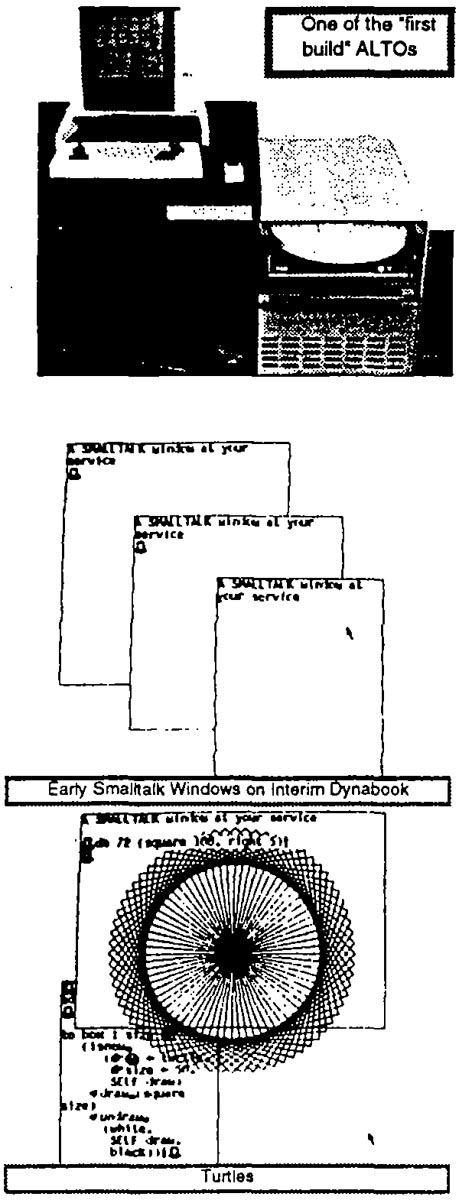
\includegraphics[scale=0.55]{WINDOWS_AND_TURTLES.jpg}
        \caption{
                \label{fig:windows_and_turles}
                Smalltalk Overlapping Windows and the LOGO Turtle.
        }
\end{figure}

\subsubsection{The Evolution of Smalltalk-72: Smalltalk-74}

Smalltalk-74 was a version of Smalltalk-72 incorporating major improvements which included providing a real "messenger" object, message dictionaries for classes (a step towards real class objects), Diana Merry's bitblt (the now famous 2D graphics operator for bitmap graphics) and a better, more general window interface.

Since the ALTO was very small storage wise, the crowning addition was the \textbf{OOZE} (Object Oriented Zoned Environment) virtual memory system. The basic idea in all of these systems is to be able to gather the most comprehensive possible working set of objects. This is most easily accomplished by swapping individual objects. Now the problem becomes the overhead of purging non-working set objects to make room for the ones that are needed.

Two ideas help a lot. First, Butler's insight in the GENIE OS that it was worthwhile to expend a small percentage of time purging dirty objects to make core as clean as possible. Thus crashes tend not to hurt as much and there is always clean storage to fetch pages or objects from the disk into. The other problem that had to be taken care of was object-pointer integrity. For this, we decided to control storage using a Resident Object Table that was the only place machine addresses for objects would be found. The key to the design was the checkpointing scheme they came up with. This insured that there always was a recoverable image no more than a few seconds old.

\subsubsection{"Object-oriented" Style}

This is probably a good place to comment on the difference between what we thought of as OOP-style and the superficial encapsulation called "abstract data types". In our opinion, the last thing you wanted any programmer to do is mess with internal state even if presented figuratively. Instead, the objects should be presented as sites of higher level behaviors more appropriate for use as dynamic components.

Where does the special efficiency of object-oriented design come from?  Part of the effect comes from a much clearer way to represent a complex system. Here, the constraints are as useful as the generalities. Four techniques used together—persistent state, polymorphism, instantiation, and methods-as-goals for the object—account for much of the power.

However, the most important principle is that when you give someone a structure, rarely do you want them to have unlimited privileges with it. Just doing type-matching isn't even close to what's needed. Nor is it terribly useful to have some objects protected and others not. Make them all first class citizens and protect all. 

\subsubsection{Smalltalk and Children}

After a failed experiment making the children draw pictures with the LOGO turtle, Adele came up with a brilliant approach to teaching Smalltalk as an object-oriented language: \textbf{the "Joe Book"}. Several instances of the class box are created and sent messages, culminating with a simple multiprocess animation. After getting kids to guess what a box might be like—they could come surprisingly close—they would be shown (like in \ref{fig:joe_book}).

It was amazing seeing the myriad of children's projects that could spring off the humble boxes, with some of them being tools! Looking back, this could be called another example of the "early success syndrome." The successes were real, but they weren't as general as we thought. \textbf{We seemed to be incubating a problem of \textit{design}}. Adults could get through the initial material faster than children, but would crash on problems that required very non intuitive building ideas.

The connection to literacy was painfully clear. It isn't enough to just learn to read and write. There is also a \textit{literature that renders ideas}. We decided we should teach design, introducing an intermediary between the vague ideas about the problem and the very detailed writing and debugging that had to be done to get it to run in Smalltalk: \textbf{Design Templates}.

Using these the children could look at a situation they wanted to simulate, and decompose it into classes and messages without having to worry just how a method would work. The method planning could then be done informally in English, and these notes would later serve as commentaries and guides to the writing of the actual code. However, it is hard to claim success if only some of the children are successful—and if a maximum effort of both children and teachers was required to get the successes to happen.

The main problem is not to get the kids to do stuff (they love that). \textbf{What is difficult is to determine what ideas to put forth and how deeply they should penetrate at a given child's developmental level}.

Should we even try to teach programming? I have met hundreds of programmers and can see no discernible influence of programming on their general ability to think well. The first siren's song we need to be wary of is the one that promises a connection between an interesting pursuit and interesting thoughts. \textbf{Tools provide a path, a context, and almost an excuse for developing enlightenment, but no tool ever contained it or can dispense it.}

Another way to look at this is that \textbf{knowledge is in its least interesting state when it is first being learned}. The representations —whether markings or physical controls— get in the way and must be interpreted. From here there are several useful paths.

The first is \textbf{fluency}, which in part is \textbf{the process of building mental structures that disappear the interpretation of the representations}. The letters and words of a sentence are experienced as meaning rather than markings, for example. One eventually becomes a kind of expert (but without deep knowledge in other areas). So, attempts to generalize are usually too crisp and ill formed.

The second path is towards \textbf{taking the knowledge as a metaphor than can illuminate other areas}. But without fluency it is more likely that prior knowledge will hold sway and the metaphors from this side will be fuzzy and misleading.

\textbf{The "trick" is to get fluent and deep while building relationships with other fluent deep knowledge}. Our society has lowered its aims so far that it is happy with "increases in scores" without daring to inquire whether any important threshold has been crossed. 

The reason, therefore, that many of us want children to understand computing deeply and fluently is that like literature, mathematics, science, art, etc it carries special ways of thinking about situations that in contrast with other knowledge and other ways of thinking critically boost our ability to understand our world. 

 \begin{figure}[ht]
        \centering 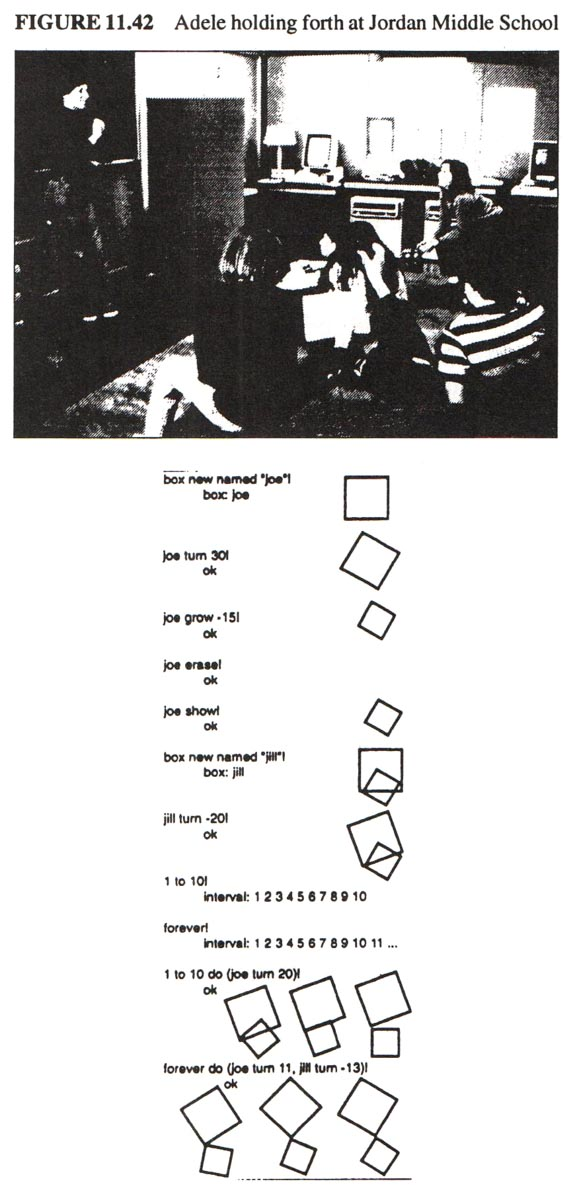
\includegraphics[scale=0.55]{JOE_BOOK.jpg}
        \caption{
                \label{fig:joe_book}
                Adele at Jordan Middle School and below, an example program of the Joe Book.
        }
\end{figure}

\subsection{1976-80: The first modern Smalltalk (-76), its birth, applications, and improvements}

When I looked at Smalltalk in 1975, I was looking at something great, but I did not see an enduser language, I did not see a solution to the original goal of a "reading" and "writing" computer medium for children.

Dan was proceeding with his total revamp of Smalltalk and along somewhat similar lines. There were a variety of strong desires for a real inheritance mechanism. Dan had to find a better way than Simula's very rigid compile-time conception. It was time to make good on the idea that "everything was an object," which included all the internal "systems" objects like "activation records," etc. We were all agreed that the flexible syntax of the earlier Smalltalks was too flexible, and this level of extensibility was not desirable. All of the extensions we liked used various keyword schemes, so Dan came up with a combination keyword/operator syntax that was very flexible, but allowed the language to be read unambiguously by both humans and the machine. This allowed a FLEX machine-like byte-code compiler and efficient interpreter to be defined that ran up to 180 times as fast as the previous direct interpreter. 

\subsubsection{Inheritance}

By the time Smalltalk-76 came along, Dan Ingalls had come up with a scheme that was Simula-like in its semantics but could be incrementally changed on the fly to be in accord with our goals of close interaction. I was not completely thrilled with it because it seemed that we needed a better theory about inheritance entirely (and still do). For example, inheritance and instancing (which is a kind of inheritance) muddles both pragmatics (such as factoring code to save space) and semantics (used for way too many tasks such as: specialization, generalization, speciation, etc.). Borning employed a multiple inheritance scheme which was implemented in Smalltalk-76. But no comprehensive and clean multiple inheritance scheme appeared that was compelling enough to surmount Dan's original Simula-like design. 
 
 \subsubsection{The Smalltalk User Interface}
 
The interface focus was on children. We were thinking about learning as being one of the main effects we wanted to have happen. This led to a 90 degree rotation of the purpose of the user interface from "access to functionality" to "environment in which users learn by doing."

The particular aim of LRG was to find the equivalent of writing. That is, learning and thinking by doing in a medium,our new "pocket universe." For various reasons I had settled on "iconic programming" as the way to achieve this, drawing on the iconic representations used by many ARPA projects in the sixties. This would allow us to be in a free environment, where exploration caused desired sequences to happen.

\subsubsection{Smalltalk-76}
An example of the Smalltalk-76 Interface can be found in \ref{fig:smalltalk76ui}. One of the iconic Smalltalk 76 classes was the  Window. With this new version,  the code is expressed as goals for other objects (or itself) to achieve.

 \begin{figure}[ht]
        \centering 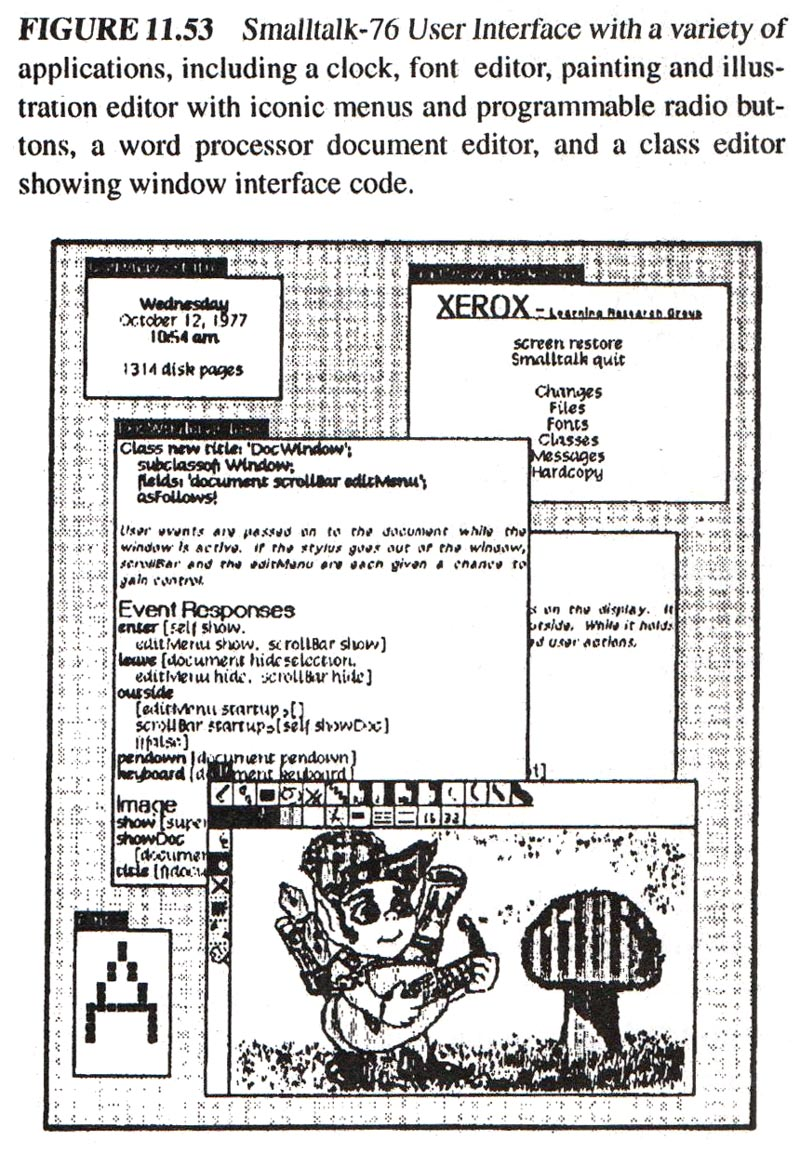
\includegraphics[scale=0.55]{SMALLTALK76_UI.jpg}
        \caption{
                \label{fig:smalltalk76ui}
                Smalltalk-76 UI
        }
\end{figure}

We later made the Smalltalk Simkit, Smalltalk-76 rich system especially tailored for adult nonexpert users. For that, we built a user interface for a generalized job shop simulation tool that the executives could make into specific dynamic simulations that would act out their changing states by animating graphics on the screen.

There were many interesting problems to be solved. The system itself was straightforward but it had to be completely sealed off from Smalltalk proper, particularly with regard to error messages. Dave Robson came up with a nice scheme (almost an expert system) to capture complaints from the bowels of Smalltalk and translated them into meaningful SimKit terms.

Meanwhile, the NoteTaker was getting more real, bigger, and slower. By this time the Western Digital emulation-style chips I hoped to used showed signs of being "diffusion-ware," and did not look like they would really show up. We started looking around for something that we could count on, even if it didn't have a good architecture.

\subsection{1980-83: The release version of Smalltalk (-80)}
\subsubsection{Coda}

\begin{thebibliography}{99}

\bibitem{EARLY_HISTORY_OF_SMALLTALK}
Alan Kay, \href{http://worrydream.com/EarlyHistoryOfSmalltalk}{Early History of Smalltalk}

\bibitem{NO_SILVER_BULLET}
Frederick P. Brooks Jr, \href{http://worrydream.com/refs/Brooks-NoSilverBullet.pdf}{No Silver Bullet}

\bibitem{MYTHICAL_MAN_MONTH}
Fred Brooks, \href{https://www.cs.drexel.edu/~yfcai/CS451/RequiredReadings/MythicalManMonth.pdf}{Mythical Man Month}

\end{thebibliography}


\end{document}
